% !TEX root = perelman-geometry.tex
%!TEX TS-program = pdflatex
%!TEX encoding = UTF-8 Unicode



\setchapterpreamble[o]{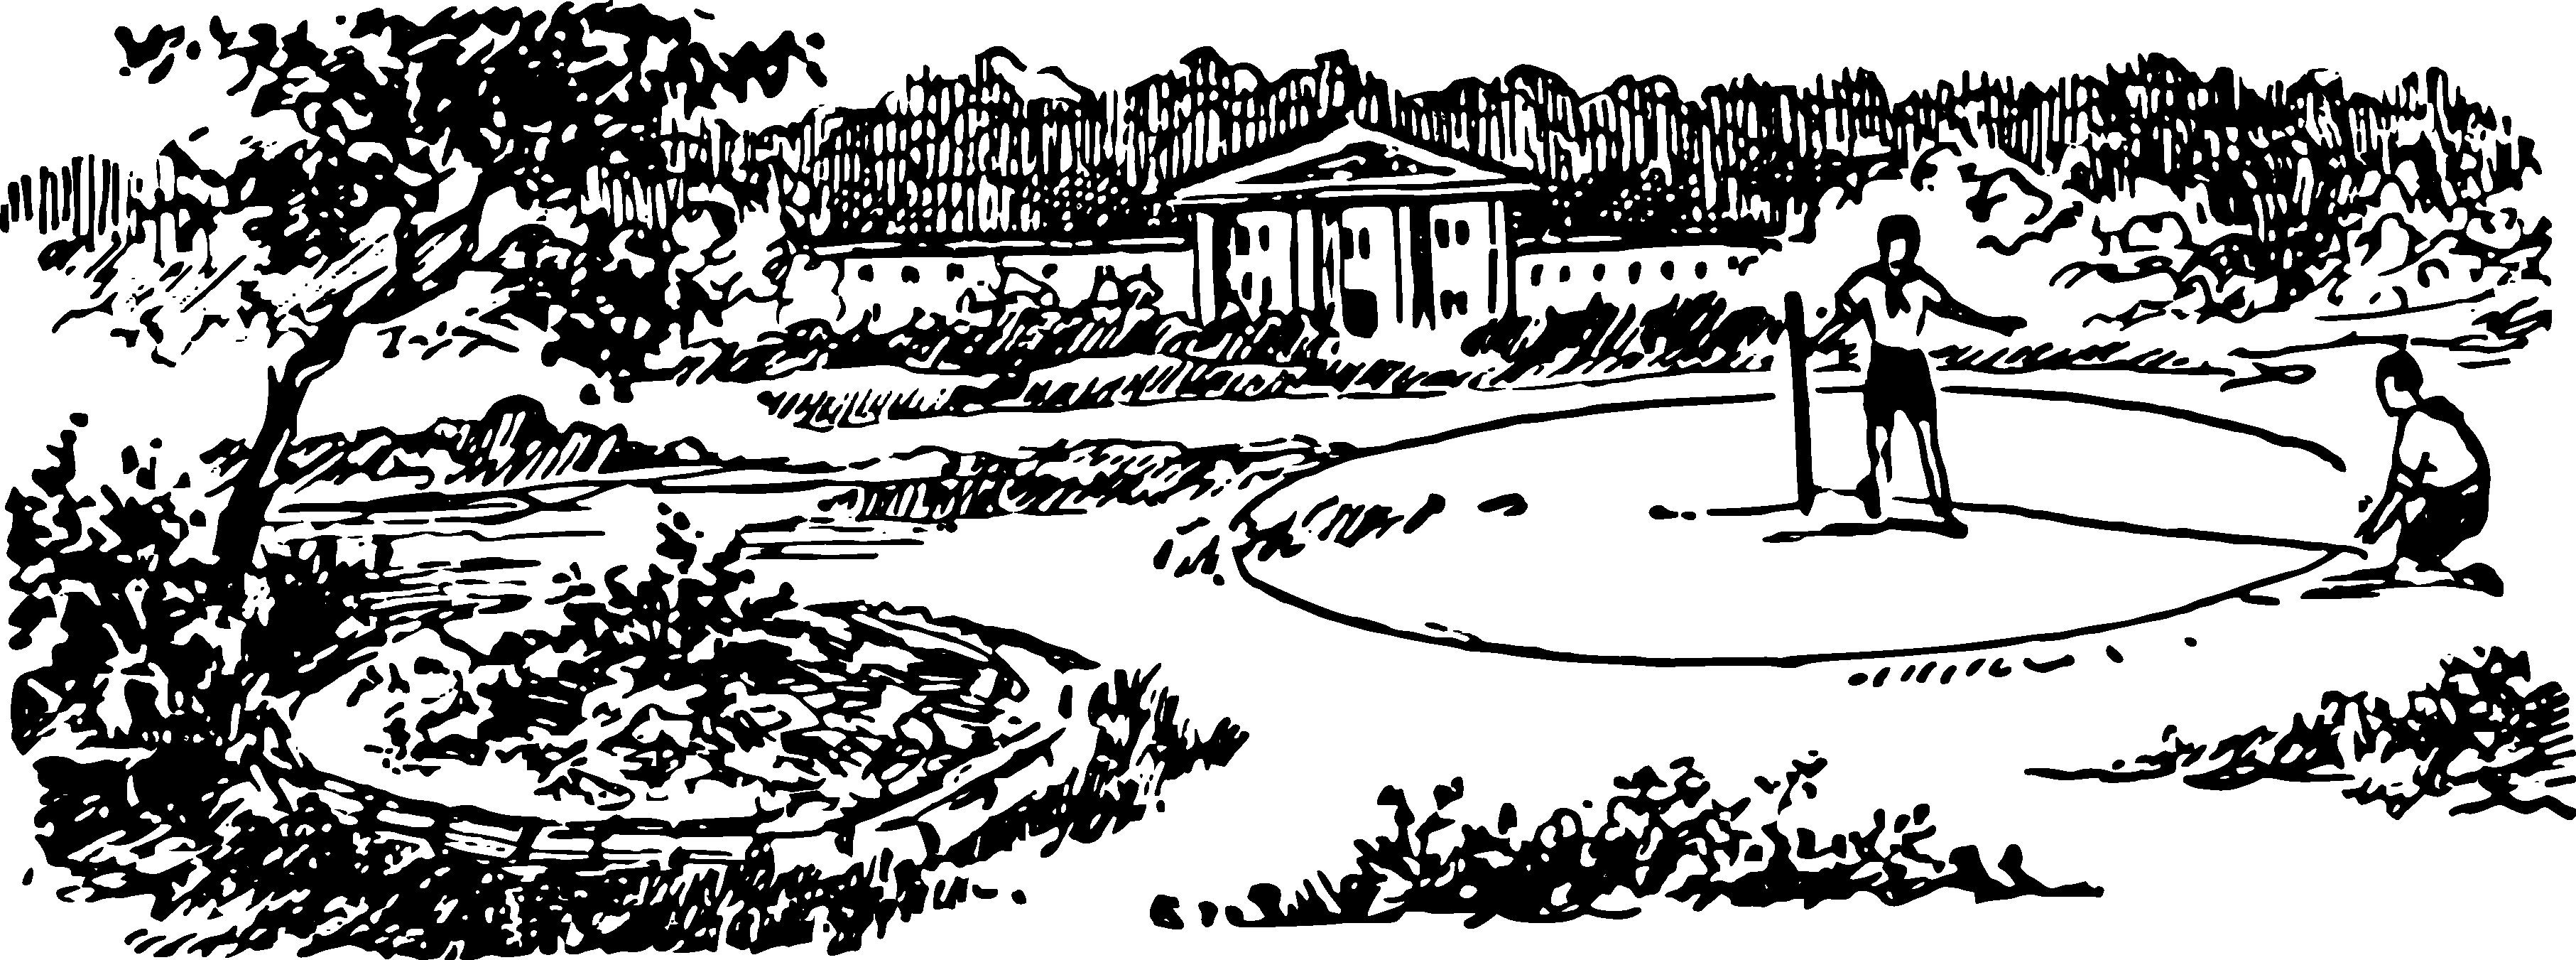
\includegraphics[width=1.2\textwidth]{figures/ch-12/fig-ch-12-head.pdf}\bigskip}

\chapter{Geometric Economy}
\label{ch-12}



\section[How Did Pahom Buy Land]{How Did Pahom Buy Land (Leo Tolstoy's Task)}
\label{sec-12.1}

We will begin this chapter, whose unusual title will become clear to the reader later on, with an excerpt from Leo Tolstoy's well-known story \emph{How Much Land Does a Man Need?}


``And what will the price be?'' Pakhom asks.

``The price is the same for everyone: 1000 roubles for a day.''

Pakhom didn’t understand.

``What kind of measure is a day? How many desyatinas\sidenote{A unit of land area. -- \textsc{dm}} is that?''

``We don't know how to count that way. We sell by the day; however much you can walk around in a day, that's yours, and the price is 1000 roubles.''

Pakhom was astonished.

``But you can walk around a lot of land in a day,'' he says.

The chief laughed.

``It's all yours,'' he says. ``But there's one condition: if you don’t return by sunset to the place where you started, you lose your money.''

``How will I mark the places I walk?'' Pakhom asks.

``We’ll stand at the place you choose to start from; we’ll stay there, and you go, make a circle, and take a scraper with you to mark where necessary, dig small holes, lay down turf at the corners; later, we'll plow from hole to hole. Choose any circle you want, but you must return to the starting place by sunset. Whatever you circle will be yours.''

The Bashkirs dispersed. They promised to gather at dawn the next day and head to the place before sunrise.

They arrived in the steppe as dawn was breaking. The chief approached Pakhom and pointed with his hand.

``Here'', he said, ``everything you can see is ours. Choose any part.''

The chief took off his fox fur hat and placed it on the ground.

``This will be the marker'', he said. ``Start from here and come back to here. Whatever you circle will be yours''.

As soon as the sun's rose, Pakhom slung the scraper over his shoulder and set off into the steppe.

He walked about a mile, stopped, and dug a small hole. He continued walking. After covering another mile, he dug another hole.

He had walked about five miles. He looked at the sun; it was already breakfast time. ``One stretch is done,'' thought Pakhom. ``And there are four stretches in a day, it’s too early to turn yet. I’ll walk another five versts and then start turning left.'' He continued straight ahead. 

``Well'', he thought, ``I’ve covered enough ground in this direction; it’s time to turn.’ He stopped, dug a larger hole, and turned sharply to the left.''

He walked a long way along this side as well, then turned the second corner. Pakhom glanced back at the shikhan (hill): it was hazy from the heat, and through the haze, he could barely see the people on the shikhan. 

``Well'', he thought, ``I've taken long sides, I need to make this one shorter''. He started on the third side. He looked at the sun—it was already nearing midday, and he had only covered about two versts on the third side. And the distance back to the starting point was still about 15 versts. 

``No'', he thought, ``even if it’s a crooked plot, I need to go straight to make it in time.''

Pakhom quickly dug a hole and turned straight towards the shikhan.

Pakhom walked straight towards the shikhan, and it was becoming hard for him. He wanted to rest but couldn’t -- he wouldn’t make it back before sunset. And the sun was already close to the horizon.

\begin{figure}[h!]
\centering
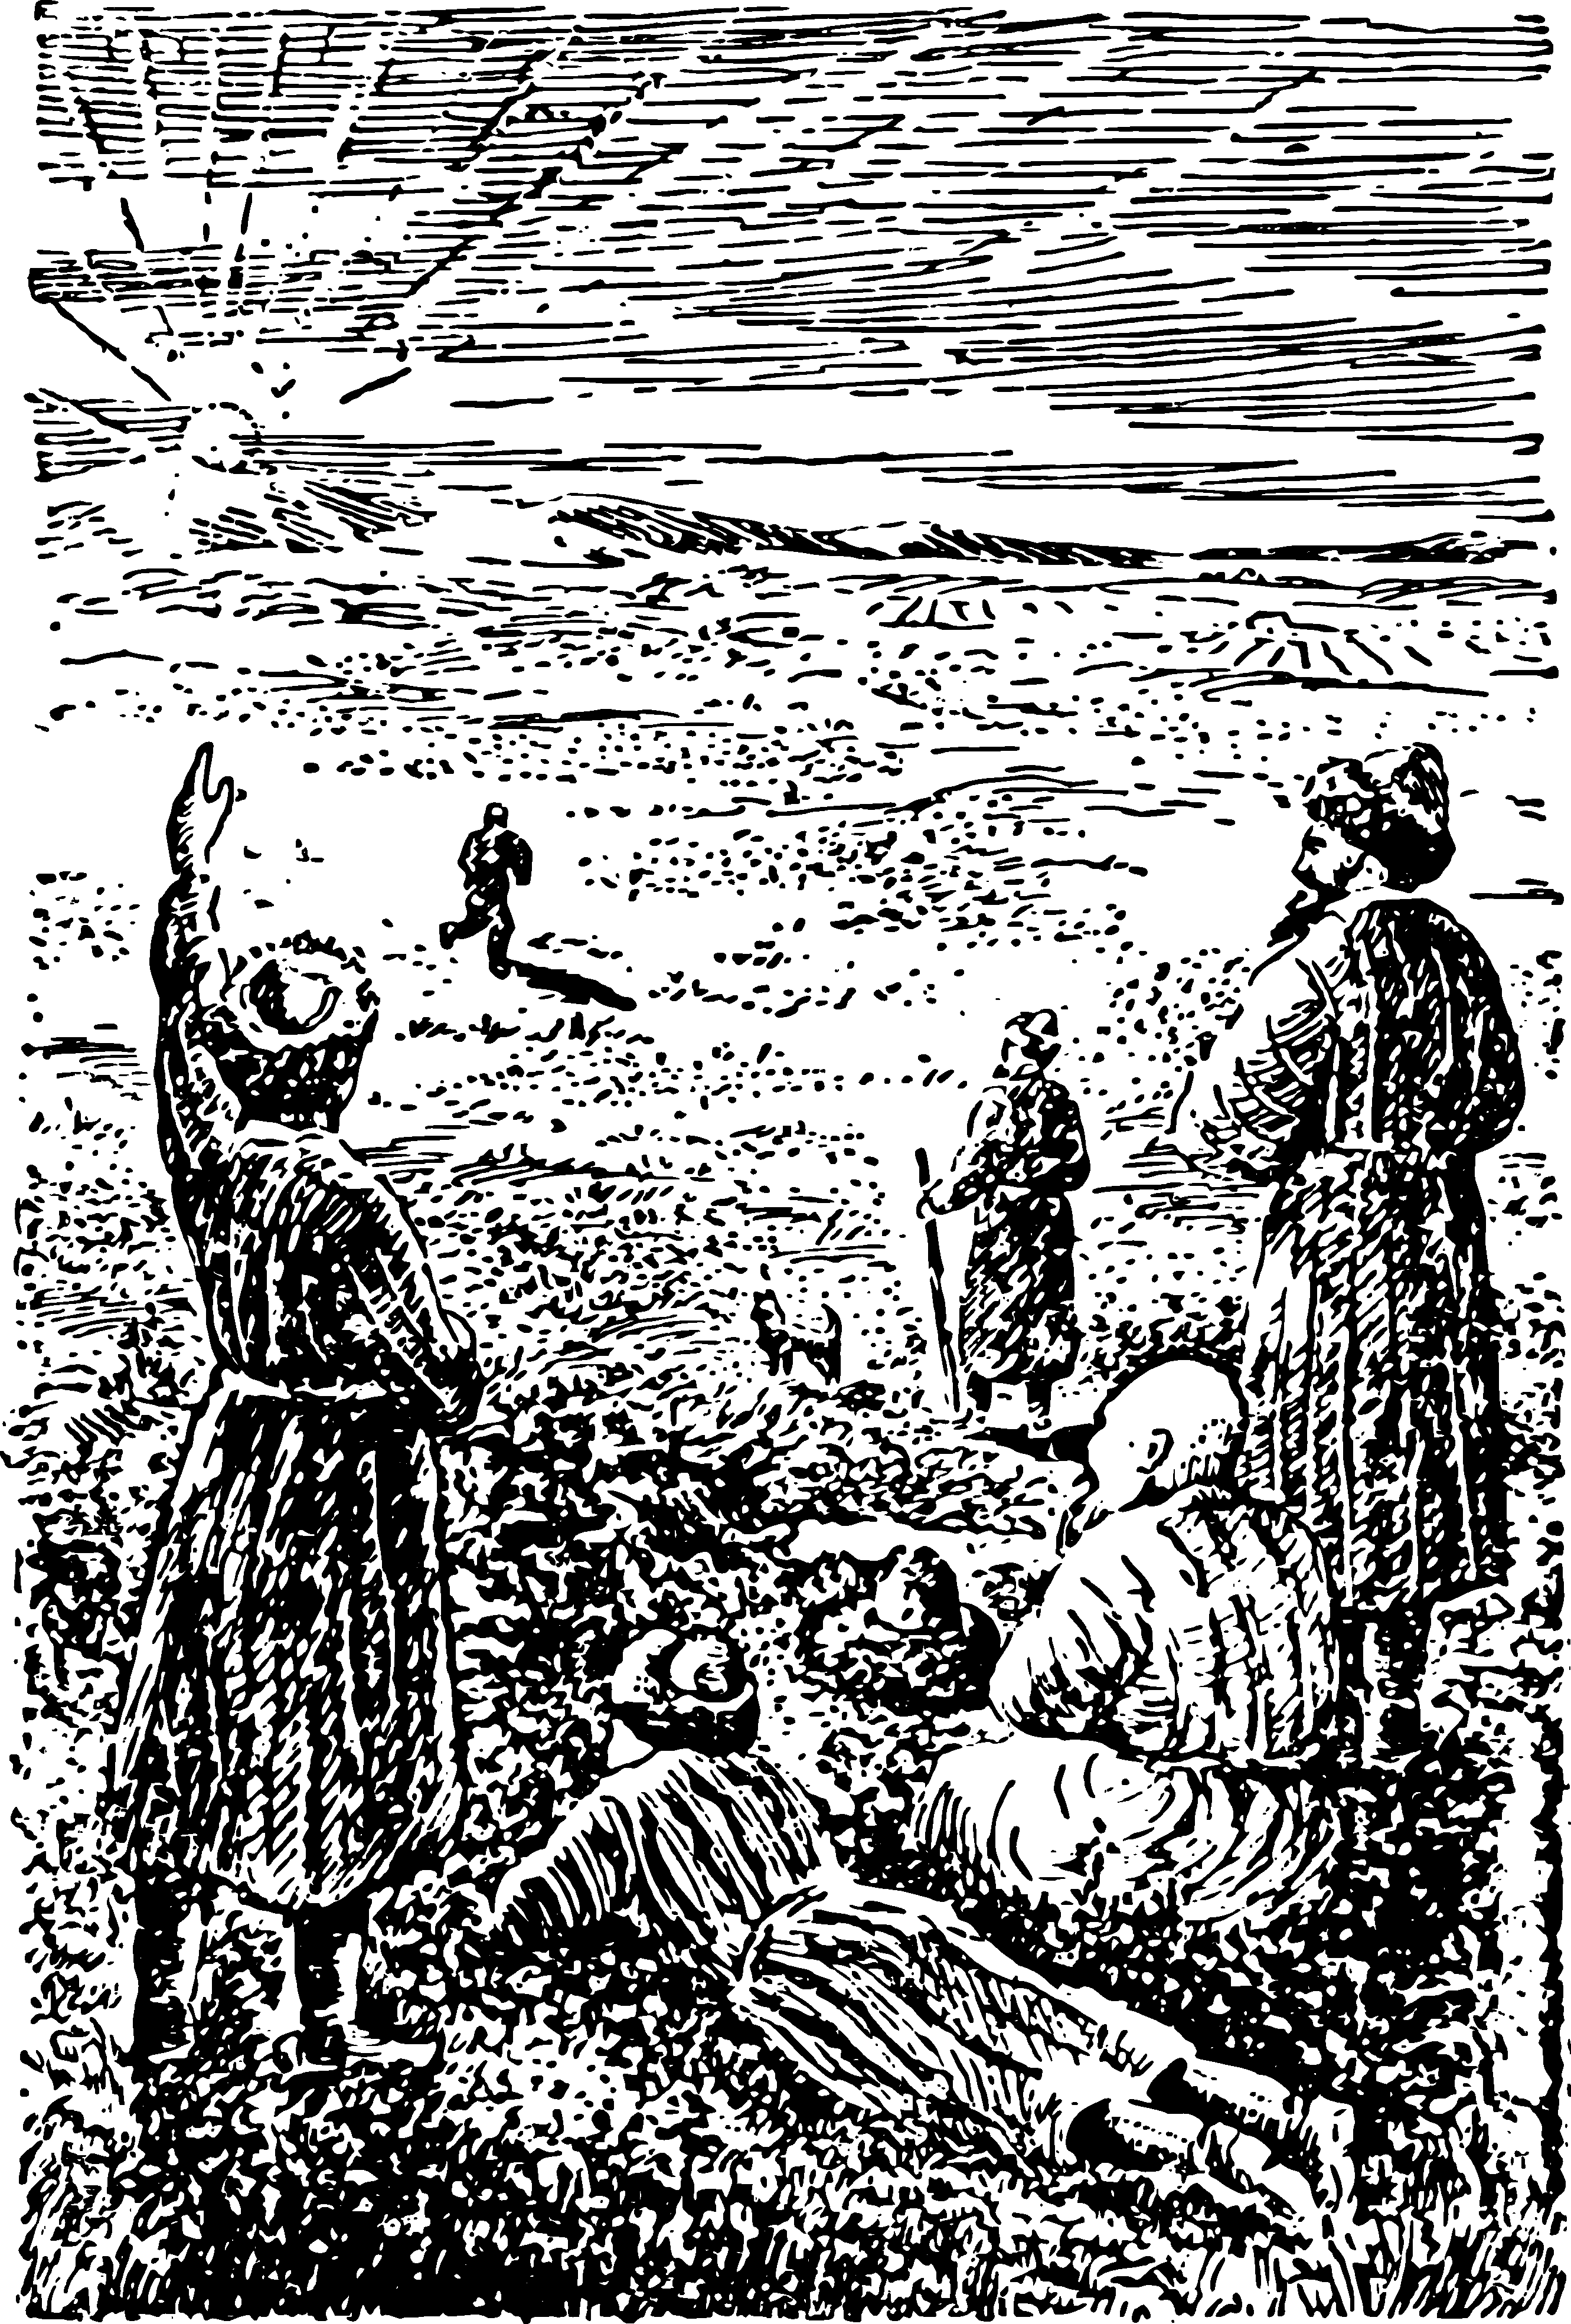
\includegraphics[width=0.7\textwidth]{figures/ch-12/fig-174.pdf}
\sidecaption{Pakhom ran with his last strength, and the sun was already near the horizon.\label{fig-174}}
\end{figure}

Pakhom kept walking, finding it increasingly difficult, but still quickening his pace. He walked and walked—still far to go; then he began to trot\dots{} Pakhom ran, his shirt and trousers sticking to his sweaty body, his mouth dry. His chest heaved like a blacksmith’s bellows, and his heart pounded like a hammer.

Pakhom ran with his last strength, and the sun was just about to set. Any moment now it would start disappearing (see \figr{fig-174}).

The sun was close, and the place was also very near. He saw the fox fur hat on the ground and the chief sitting on the ground.




Pakhom looked at the sun; it had already touched the ground and was just starting to set. Summoning his last bit of strength, Pakhom pushed himself, gathered his breath, and ran up the shikhan. He saw the hat. His legs gave way, and he fell forward, reaching the hat with his hands.

``Well done!'' shouted the chief. ``You have acquired a lot of land''.

An assistant ran up, trying to lift him, but blood was flowing from Pakhom's mouth, and he lay there dead\dots{}


\section{The Problem of Leo Tolstoy}
\label{sec-12.2}

Let's set aside the grim conclusion of this story and focus on its geometric aspect. Is it possible to determine, based on the scattered information in this story, approximately how many desyatinas of land Pakhom walked around? The task, which at first glance seems impossible, is actually solved quite simply.


\ans By carefully rereading the story and extracting all geometric indications, it is not difficult to convince oneself that the data provided is sufficient for a comprehensive answer to the question. One can even draw a plan of the land parcel that Pakhom walked around.

First of all, it is clear from the story that Pakhom ran along the sides of a quadrilateral. Regarding the first side, we read:

``He walked about five versts\dots{} \quad ``I’ll go another five versts, then I’ll turn left\dots{}''

Thus, the first side of the quadrilateral was about 10 versts long.

For the second side, which forms a right angle with the first, no numerical indications are given in the story.

The length of the third side, evidently perpendicular to the second, is directly stated in the story: ``Along the third side, he had walked only about two versts.''

``The length of the third side—clearly perpendicular to the second—is directly stated in the story: 'Along the third side, he had walked only about two versts.'

The length of the fourth side is also directly provided: ``To the place it is still the same 15 versts.''\sidenote{It is unclear here how Pakhom could see people on the hill from such a distance.}



Using this data, we can draw the plan of the land parcel that Pakhom walked around (see \figr{fig-175}). In the resulting quadrilateral $ABCD$, the side $AB = 10$ versts; $CD = 2$ versts; $AD = 15$ versts; and angles $B$ and $C$ are right angles. The length $x$ of the unknown side $BC$ can be easily calculated by drawing the perpendicular $DE$ from $D$ to $AB$ (see \figr{fig-176}). Then in the right triangle $AED$, we know the leg $AE = 8$ versts and the hypotenuse $AD = 15$ versts. The unknown leg $ED = \sqrt{15^{2} - 8^{2}} = 13$ versts.
\begin{marginfigure}[-2cm]%[h!]
\centering
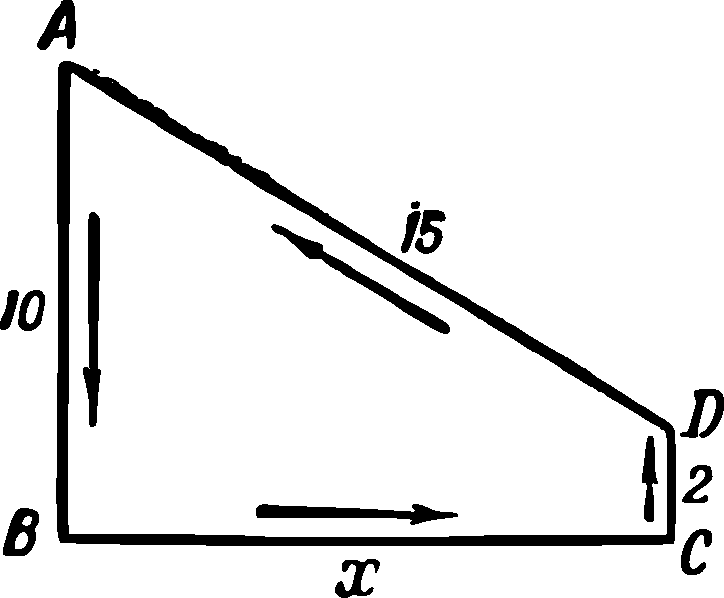
\includegraphics[width=\textwidth]{figures/ch-12/fig-175.pdf}
\sidecaption{Tracing Pakhom’s route.\label{fig-175}}
\end{marginfigure}


So, the second side was about 13 versts long. Obviously, Pakhom was mistaken, thinking the second side was shorter than the first.

\begin{marginfigure}[2cm]%[h!]
\centering
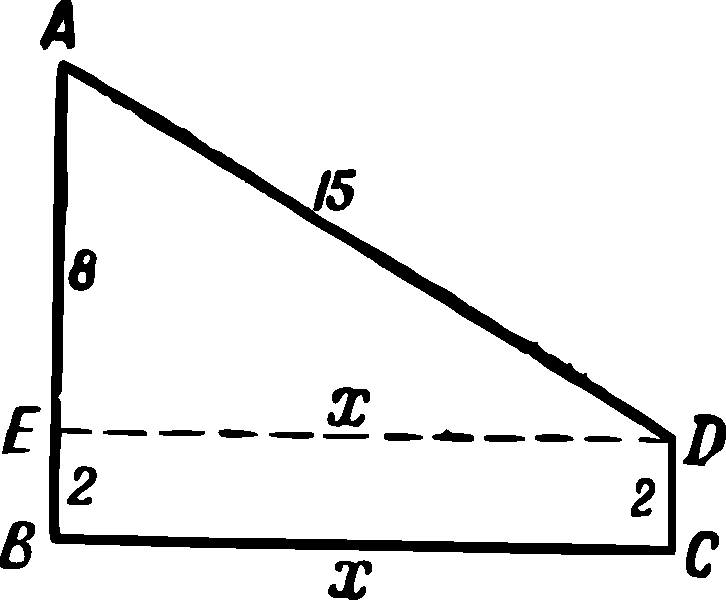
\includegraphics[width=\textwidth]{figures/ch-12/fig-176.pdf}
\sidecaption{Pakhom’s route clarification.\label{fig-176}}
\end{marginfigure}

As you can see, it is quite possible to accurately draw the plan of the area Pakhom walked around. Undoubtedly, L.N.~Tolstoy had a drawing similar to \figr{fig-175} in front of him when writing his story.

Now it is easy to calculate the area of the trapezoid $ABCD$, consisting of the rectangle $EBCD$ and the right triangle $AED$. It equals:
\begin{equation*}%
2 \times 13 + \frac{1}{2} \times 8 \times 13 = 78 \,\,\text{square versts}.
\end{equation*}
Calculating using the trapezoid formula would, of course, give the same result:
\begin{equation*}%
\frac{(AB + CD)}{2} \times BC = \frac{(10 + 2)}{2} \times 13  = 78 \,\,\text{square versts}.
\end{equation*}
We have determined that Pakhom walked around a vast area of 78 square versts, or about 8000 desyatinas. Each desyatin cost him 12.5 kopecks.

\section{Trapezoid or Rectangle}
\label{sec-12.3}


\ques On the fateful day of his life, Pakhom walked $10 + 13 + 2 + 15 = 40$ versts along the sides of a trapezoid. His initial intention was to walk along the sides of a rectangle; the trapezoid resulted accidentally due to poor calculation. It is interesting to determine whether he gained or lost from the fact that his plot turned out to be a trapezoid rather than a rectangle. In which case would he have obtained a larger area of land?

\ques Rectangles with a perimeter of 40 versts can vary widely, each having a different area. Here are several examples:
\begin{align*}%
14 \times 6 & = 84 \,\, \text{square versts}\\
13 \times 7 & = 91 \\
12 \times 8 & = 96 \\
11 \times 9 & = 99
\end{align*}
We see that all these figures, with the same perimeter of 40 versts, have a larger area than our trapezoid. However, there can also be rectangles with a perimeter of 40 versts whose area is smaller than that of the trapezoid:
\begin{align*}%
18 \times 2 & = 36 \,\, \text{square versts}\\
19 \times 1 & = 19 \\
19.5 \times 0.5 & = 9.75
\end{align*}
Therefore, we cannot give a definitive answer to the problem. There are rectangles with a larger area than the trapezoid, but there are also rectangles with a smaller area, given the same perimeter. However, we can definitively answer the question: which rectangle with a given perimeter encloses the largest area? Comparing our rectangles, we notice that the smaller the difference in the length of the sides, the larger the area of the rectangle. It is natural to conclude that when there is no difference at all, i.e., when the rectangle becomes a square, the area of the figure reaches its maximum. It will then be $10 \times 10 = 100$ square versts. It is easy to see that this square indeed exceeds in area any rectangle with the same perimeter. Pakhom should have walked along the sides of a square to obtain the largest plot of land -- 22 square versts more than what he managed to encompass.


\section{The Remarkable Property of a Square}
\label{sec-12.4}

The remarkable property of a square -- enclosing the largest area compared to all other rectangles with the same perimeter -- is not widely known. Therefore, let's provide a rigorous proof of this statement.

Let's denote the perimeter of a rectangular figure by \( P \). If we take a square with this perimeter, then each side must be \( P/4 \). We will prove that by shortening one side of the square by some amount \( b \) while lengthening the adjacent side by the same amount, we get a rectangle with the same perimeter but a smaller area. In other words, we will prove that the area of the square \( (P/4)^{2} \) is greater than the area of the rectangle \( (P/4 - b)(P/4 + b) \):
\begin{equation*}%
 (P/4)^{2} > (P/4 - b)(P/4 + b).
\end{equation*}
Since the right side of this inequality equals \( (P/4)^{2} - b^{2} \), the entire expression becomes:
\begin{equation*}%
 0 > -b^{2} \qor b^{2} > 0 
\end{equation*}
But the latter inequality is obvious: the square of any number, whether positive or negative, is greater than 0. Therefore, the initial inequality, which led us to this conclusion, is also true.

Thus, a square has the largest area of all rectangles with the same perimeter.

This implies, among other things, that of all rectangular figures with equal areas, the square has the smallest perimeter. We can confirm this through the following reasoning. Suppose this is not true and there exists a rectangle $A$, which has an equal area to square $B$ but a smaller perimeter. Then, by drawing a square $C$ with the same perimeter as rectangle $A$, we would get a square with a larger area than $A$, and therefore larger than square $B$. What do we have as a result? That square $C$ has a smaller perimeter than square $B$ but a larger area. This is clearly impossible: if the side of square $C$ is smaller than the side of square $B$, its area must also be smaller. Hence, it was not possible to assume the existence of rectangle $A$, which, with equal area, has a smaller perimeter than a square. In other words, of all rectangles with the same area, the square has the smallest perimeter.

Familiarity with these properties of the square would have helped Pakhom correctly calculate his strength and obtain a rectangular plot of the largest area. Knowing that he could walk 36 versts in a day without strain, he would have followed the boundary of a square with a side of 9 versts and by evening would have owned a plot of 81 square versts, 3 square versts more than he acquired with fatal exertion. Conversely, if he had initially limited himself to a specific area of a rectangular plot, say 36 square versts, he could have achieved the result with the least effort by following the boundary of a square with a side of 6 versts.

\section{Plots of Different Shapes}
\label{sec-12.5}

But perhaps it would have been even more advantageous for Pakhom to carve out a plot of land not in a rectangular shape, but in some other form—quadrilateral, triangular, pentagonal, etc.?

This question can be considered strictly mathematically; however, out of concern for tiring our voluntary reader, we will not delve into this consideration here and will only acquaint him with the results.

Firstly, it can be proven that of \emph{all quadrilaterals} with equal perimeter, the square has the largest area. Therefore, in seeking to have a quadrilateral plot, Pakhom could not have acquired more than 100 square versts by any means (assuming his maximum daily walk was 40 versts).

Secondly, it can be proven that a square has a larger area than any triangle of equal perimeter. An equilateral triangle with the same perimeter would have a side of 40/3 = 13 \, 1/3 versts, and its area (using the formula \( S = \frac{a^{2} \sqrt{3}}{4} \), where \( S \) is the area and \( a \) is the side) would be:
\begin{equation*}%
 S = \frac{1}{4} \left(\frac{40}{3}\right)^{2} \sqrt{3} = 77 \,\, \text{ square versts}.
 \end{equation*}
"i.e., even less than that of the trapezoid Pakhom walked around. Further (on page~\pageref{sec-10.2}), it will be proven that of all triangles with equal perimeters, the scalene triangle has the largest area. This means that if even the largest triangle has an area smaller than that of the square, then all other triangles with the same perimeter will have areas smaller than the square.

But if we compare the area of the square with that of a pentagon, hexagon, etc., with the same perimeter, the square's supremacy ends here: a regular pentagon has a larger area, a regular hexagon even larger, and so on. This can be easily verified with the example of a regular hexagon. With a perimeter of 40 versts, the side of the hexagon is 40/6 versts, and its area (using the formula \( S = (3a^{2}\sqrt{3})/2 \) is:
\begin{equation*}%
 \frac{3}{2} \left(\frac{40}{6}\right)^{2} \sqrt{3} = 115 \,\, \text{ square versts}.
 \end{equation*}
If Pakhom had chosen a regular hexagon for his plot, he would have acquired an area 115 - 78, i.e., 37 square versts more than he actually did, and 15 square versts more than he would have gotten from a square plot. (However, to achieve this, he would have needed to embark on his journey with surveying instruments).



\ques Arrange six matches to form a figure with the largest possible area.


\ans With six matches, one can create a variety of shapes: an equilateral triangle, a rectangle, numerous parallelograms, several irregular pentagons, various irregular hexagons, and finally, a regular hexagon. A geometer, without comparing the areas of these shapes, already knows which one has the largest area: a regular hexagon.


\section{Figures with the Greatest Area}
\label{sec-12.6}

It can be proven geometrically that the greater the number of sides in a regular polygonal area, the larger the area it encloses for the same boundary length. The shape with the largest area for a given perimeter is a circle. If Pakhom had run in a circle, covering the same 40 versts, he would have obtained an area of
\begin{equation*}%
 \pi \left( \frac{40}{2\pi} \right)^{2} = 127 \,\, \text{ square versts}. \end{equation*}
No other shape, whether straight-edged or curved, can have a larger area with the same perimeter.

We will take some time to focus on this remarkable property of the circle to enclose a greater area than any other figure of any shape with the same perimeter. Some readers might be curious to know how such properties are proven. Below is a proof—though not entirely rigorous—proposed by mathematician Jakob Steiner. It is quite lengthy, but those who find it tedious can skip it without losing the understanding of what follows.

\begin{marginfigure}[-3cm]%[h!]
\centering
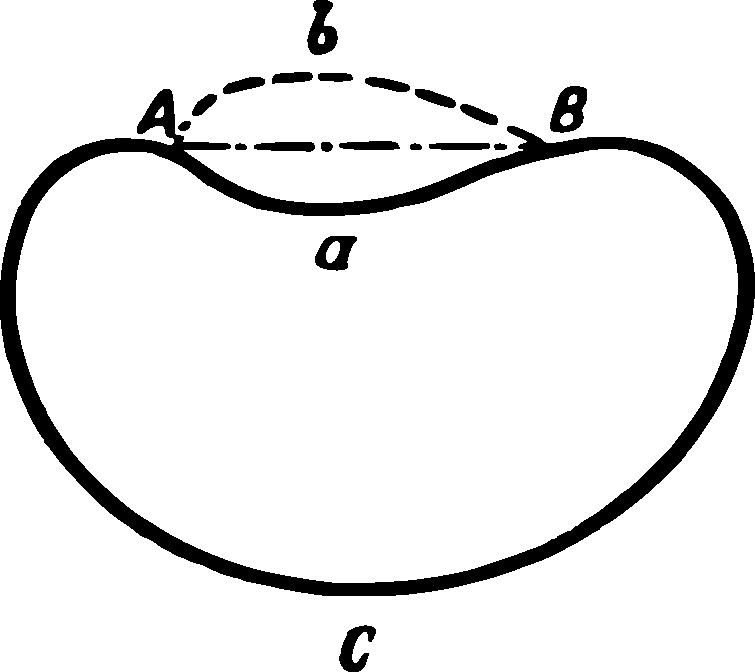
\includegraphics[width=\textwidth]{figures/ch-12/fig-177.pdf}
\sidecaption{Establishing that the figure with the maximum area must be convex.\label{fig-177}}
\end{marginfigure}

It is necessary to prove that the figure with the maximum area for a given perimeter is a circle. First, let's establish that the desired figure must be convex. This means that every chord of the figure must lie entirely inside it. Suppose we have a figure \(AaBC\) (\figr{fig-177}) with an external chord \(AB\). Let's replace the arc \(a \) with an arc \(b \), which is symmetrical to it. This replacement will not change the perimeter of the figure \(ABC\), but it will clearly increase the area. Therefore, figures like \(AaBC\) cannot be the ones that enclose the maximum area for the same perimeter.

\begin{marginfigure}[-2cm]%[h!]
\centering
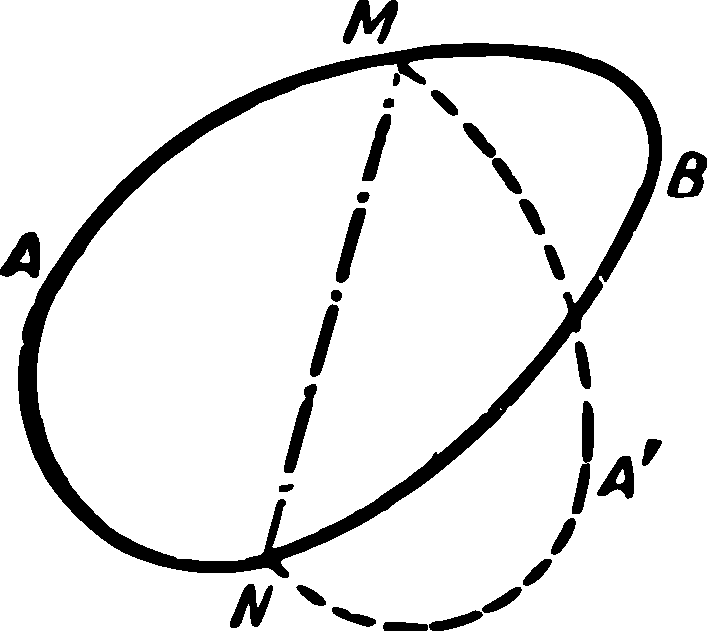
\includegraphics[width=\textwidth]{figures/ch-12/fig-178.pdf}
\sidecaption{If a chord bisects the perimeter of a convex figure with the largest area, then it bisects the area.\label{fig-178}}
\end{marginfigure}

Thus, the desired figure is convex. Furthermore, we can also establish another property of this figure: any chord that bisects its perimeter must also bisect its area. Let the figure \(AMBN\) (\figr{fig-178}) be the desired one, and let the chord \(MN\) bisect its perimeter. We need to prove that the area \(AMN\) is equal to the area \(MBN\). 



Indeed, if one of these parts were larger than the other, for example, if \(AMN > MNB\), then by folding the figure \(AMN\) along \(MN\), we would obtain the figure \(AMA'N\), whose area is larger than the original figure \(AMB'M\), while the perimeter remains the same. Therefore, the figure \(AMBN\), in which a chord bisecting the perimeter does not divide the area equally, cannot be the desired one (i.e., it cannot have the maximum area for a given perimeter).

Before proceeding further, let's prove the following auxiliary theorem: among all triangles with two given sides, the one with these sides enclosing a right angle has the greatest area. To prove this, let's recall the trigonometric expression for the area \(S\) of a triangle with sides \(a\) and \(b\) and the angle \(C\) between them:
\begin{equation*}%
S = \frac{1}{2} ab \, \sin C.
\end{equation*}
This expression is obviously maximised (for given sides) when \(\sin C\) takes its maximum value, i.e., when it equals one. But the angle whose sine is 1 is a right angle, which is what needed to be proven.

\begin{marginfigure}[-3cm]%[h!]
\centering
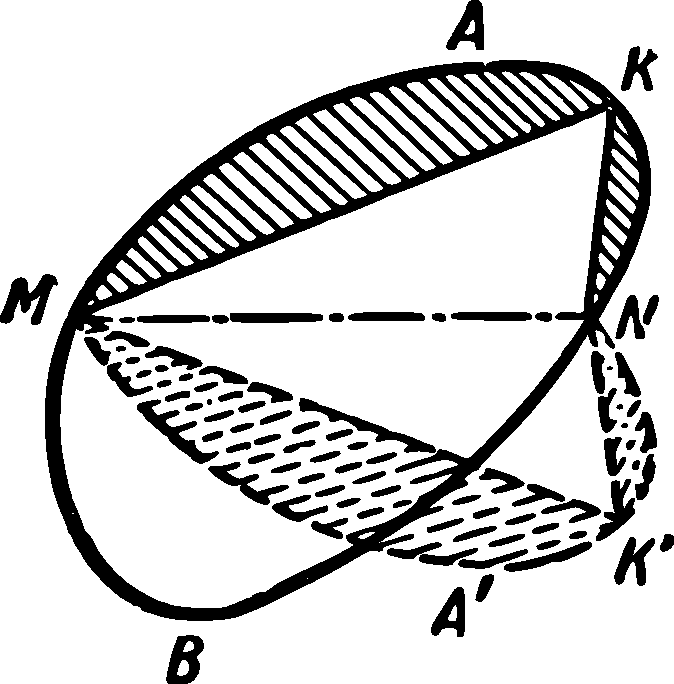
\includegraphics[width=\textwidth]{figures/ch-12/fig-179.pdf}
\sidecaption{We assume the existence of a non-circular convex shape with the largest area.\label{fig-179}}
\end{marginfigure}

Now we can proceed to the main task -- proving that among all figures with perimeter \(p\), the circle encloses the greatest area. To confirm this, let's try to assume the existence of a non-circular convex figure \(MANB\) (\figr{fig-179}) that possesses this property. Let's draw a chord \(MN\) in it, bisecting its perimeter; as we know, it will also bisect the area of the figure.




\begin{marginfigure}%[-3cm]%[h!]
\centering
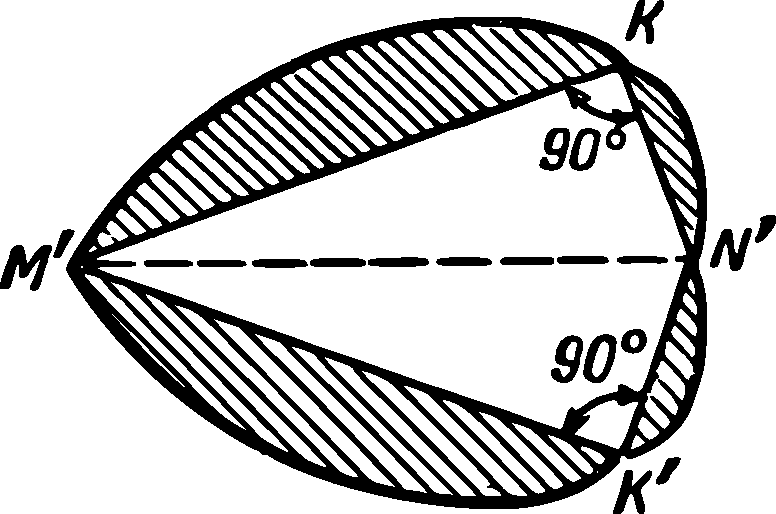
\includegraphics[width=\textwidth]{figures/ch-12/fig-180.pdf}
\sidecaption{We establish that of all the figures with a given perimeter, the largest area is limited by a circle.\label{fig-180}}
\end{marginfigure}

We will bend half of the polygon $MKN$ along the line $MN$ so that it is positioned symmetrically $(MK'N)$. Notice that the figure $MNK'M$ has the same perimeter and area as the original figure $MNKM$. Since the arc $MNK$ is not a semicircle (otherwise there would be nothing to prove), there must be points on it from which the segment $MN$ is not visible at a right angle. 

Let $K$ be such a point, and $K'$ be its symmetric point, i.e., angles $K$ and $K'$ are not right angles. By spreading (or shifting) the sides $MK$, $KN$, $MK'$, $NK'$, we can make the angle enclosed between them right, thus obtaining equal right-angled triangles. Adding these triangles along the hypotenuses, as shown in \figr{fig-180}, and attaching the shaded segments in corresponding positions, we obtain the figure $M'KMN'K'$, which has the same perimeter as the original but, obviously, a larger area (because the right-angled triangles $M'KN'$ and $M'K'N'$ have a greater area than the non-right-angled $MKN$ and $MK'N$). Therefore, no non-circular figure can have the greatest area with a given perimeter. And only in the case of a circle, using the method described, could we not construct a figure with the same perimeter and a greater area.

This is how we can prove that a circle is the figure that has the greatest area with a given perimeter.

It is easy to prove the validity of such a position: among all figures of equal area, the circle has the smallest perimeter. To do this, we need to apply to the circle the reasoning that we previously applied to the square (see page~\pageref{sec-12.4}).

\section{Nails}
\label{sec-12.7}

\ques Which nail is harder to pull out -- round, square, or triangular -- if they are driven in equally deep and have the same cross-sectional area?

\ans Let's start by assuming that the nail that has more surface area in contact with the surrounding material holds tighter. Which of our nails has the largest lateral surface area? We already know that with equal areas, the perimeter of a square is less than the perimeter of a triangle, and the circumference is less than the perimeter of a square. If we take the side of the square as one unit, then the calculation gives us the following values for these three shapes: 4.53, 4 (for triangle), and 3.55. Therefore, the triangular nail should hold tighter than the others.

However, such nails are not manufactured, at least they are not found for sale. The reason is probably that such nails are easier to bend and break.


\section{Body of Greatest Volume}
\label{sec-12.8}

Similar to the property of a circle, a spherical surface possesses the largest volume for a given surface area. Conversely, of all bodies of equal volume, the sphere has the least surface area. These properties are not devoid of significance in practical life. A spherical samovar\sidenote{A samovar is a metal container traditionally used to heat and boil water.  -- \textsc{dm}} has less surface area than a cylindrical one or one of any other shape that can hold the same number of cups. Since a body loses heat only from its surface, a spherical samovar cools down more slowly than any other of the same volume. Conversely, the reservoir of a thermometer heats up and cools down quickly (i.e., reaches the temperature of surrounding objects) when given a shape other than a sphere, such as a cylinder.

For the same reason, the Earth, consisting of a solid shell and a core, must decrease in volume, i.e., compress and become denser, due to all the factors that alter its surface shape: its internal contents must become tighter whenever its external shape undergoes any change, deviating from that of a sphere. Perhaps this geometric fact is related to earthquakes and tectonic phenomena in general, but geologists should have judgement on this.

\section{Product of Equal Factors}
\label{sec-12.9}



Problems like the ones we've been discussing approach the question from an economic perspective: given a certain expenditure of effort (for example, travelling a 40-verst distance), how can one achieve the most advantageous outcome (covering the largest area)? Hence the title of this section of the book: \emph{Geometric Economy}. However, this is a popularisation, in mathematics, questions of this kind are known by a different name: problems \emph{on maxima and minima}. They can vary greatly in plot and difficulty level. Many can only be solved using advanced mathematical techniques, but there are also many that require only elementary knowledge for their solution. Later on, a series of such problems from the field of geometry will be considered, which we will solve using one curious property of the product of equal factors.

For the case of two factors, this property is already familiar to us. We know that the area of a square is greater than the area of any rectangle with the same perimeter. If we translate this geometric statement into arithmetic language, it means the following: when it is necessary to divide a number into two parts such that their product is the greatest, one should divide it in half. For example, among all products:
\begin{equation*}%
3 \times 17, \,\,  16 \times 14,\,\,  12 \times 18, \,\, 11 \times 19, \,\,  10 \times 20, \,\,  15 \times 15
\end{equation*}
and so on, with the sum of the factors being equal to 30, the greatest product will be $15 \times 15$, even when comparing products of fractional numbers (like $14.5 \times 15.5$), and so forth.


The same applies to products of three factors having a constant sum: their product reaches its maximum value when the factors are equal to each other. This directly follows from the previous reasoning. Let three factors $x$, $y$, $z$, with a sum equal to $a$:
\begin{equation*}%
x + y + z = a.
\end{equation*}
Suppose x and y are not equal to each other. If we replace each of them with half the sum $(x + y) / 2$, the sum of the factors will not change:
\begin{equation*}%
\frac{x + y}{2} + \frac{x + y}{2} + z = x + y + z = a.
\end{equation*}
But since according to the previous reasoning
\begin{equation*}%
\frac{x + y}{2} \times\frac{x + y}{2} > xy,
\end{equation*}
then the product of the three factors
\begin{equation*}%
\frac{x + y}{2} \times\frac{x + y}{2} \times z
\end{equation*}
is greater than the product $xyz$:
\begin{equation*}%
\frac{x + y}{2} \times\frac{x + y}{2} \times z > xyz
\end{equation*}
In general, if among the factors $x$, $y$, $z$ there are at least two unequal ones, we can always find numbers that, without changing the total sum, will give a greater product than $xyz$. And only when all three factors are equal, such replacement cannot be made. Therefore, for $x + y + z = a$, the product $xyz$ will be maximum when
\begin{equation*}%
x = y = z
\end{equation*}
Let's use this property of equal factors to solve several interesting problems.

\section{Triangle with the Greatest Area}
\label{sec-12.10}



\ques What shape should a triangle have to have the greatest area given the sum of its sides?

We have already noticed earlier (page~\pageref{sec-12.2}) that this property belongs to an equilateral triangle. But how can we prove it?



\ans The area $S$ of a triangle with sides $a$, $b$, $c$ and perimeter $a + b + c = 2p$ is expressed, as known from the course of geometry, as:
\begin{equation*}%
S = \sqrt{p(p - a)(p - b)(p - c)},
\end{equation*}
from which
\begin{equation*}%
\frac{S^{2}}{p} = (p - a)(p - b)(p - c).
\end{equation*}
The area $S$ of the triangle will be maximum when its square $S^{2} $ becomes maximum, or the expression $S^{2}/p$: where $p$, the semi-perimeter, is according to the condition a constant quantity. But since both parts of the equation simultaneously achieve their maximum value, the question boils down to when the product
\begin{equation*}%
(p - a)(p - b)(p - c),
\end{equation*}
becomes maximum. Noticing that the sum of these three factors is a constant,
\begin{equation*}%
(p - a) + (p - b) + (p - c) = 3p - (a + b + c) = 3p - 2p = p,
\end{equation*}
we conclude that the product reaches its maximum value when the factors are equal, i.e., when the equality is achieved:
\begin{equation*}%
p - a = p - b = p - c
\end{equation*}
from which
\begin{equation*}%
a = b = c
\end{equation*}
Thus, a triangle has the greatest area for a given perimeter when its sides are equal to each other.

\section{The Heaviest Beam}
\label{sec-12.11}


\ques From a cylindrical log, a beam of the greatest weight needs to be cut. How can this be done?



\ans The problem, obviously, boils down to inscribing a rectangle with the greatest area in a circle. Although after all that has been said, the reader may already suspect that such a rectangle will be a square, it is still interesting to rigorously prove this proposition.


\begin{marginfigure}%[-3cm]%[h!]
\centering
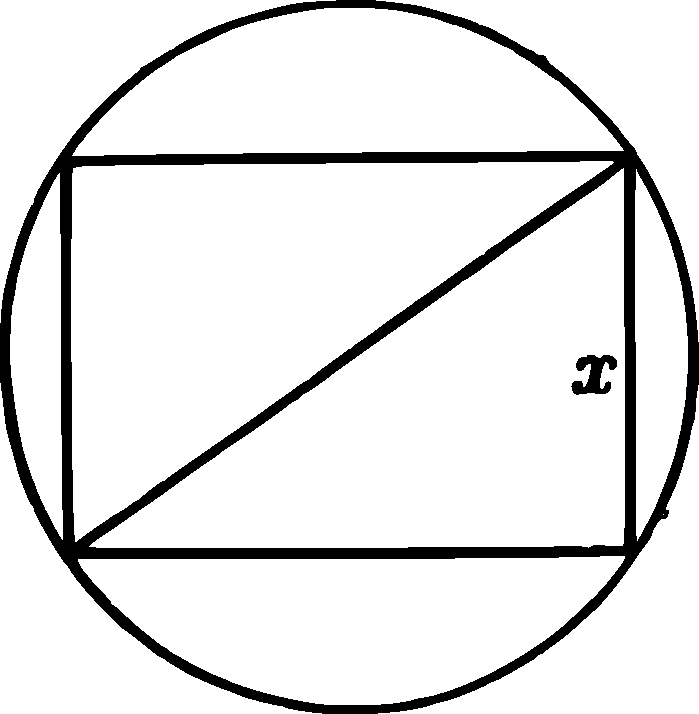
\includegraphics[width=\textwidth]{figures/ch-12/fig-181.pdf}
\sidecaption{To the problem of the heaviest beam.\label{fig-181}}
\end{marginfigure}


Let's denote one side of the sought rectangle (\figr{fig-181}) as $x$; then the other side can be expressed as $\sqrt{4R^{2} - x^{2}}$, where $R$ is the radius of the circular cross-section of the log. The area of the rectangle is $S = x\sqrt{4R^{2} - x^{2}}$ from which we get
\begin{equation*}%
S^{2} = x^{2}(4R^{2} - x^{2})
\end{equation*}
Since the sum of the factors $x^{2}$ and $4R^{2} - x^{2}$ is a constant value $(x^{2} + 4R^{2} - x^{2} = 4R^{2})$, then the product of $S^{2}$ will be maximum when $x^{2} = 4R^{2} - x^{2}$, i.e., when $x = R\sqrt{2}$. At the same time, $S$, i.e., the area of the sought rectangle, also reaches its maximum value.

Thus, one side of the rectangle with the greatest area is equal to $R\sqrt{2}	$, i.e., to the side of the inscribed square. The beam has the greatest volume when its cross-section is a square inscribed in the cross-section of the cylindrical log.


\section{From a Cardboard Triangle} 
\label{sec-12.12}


\ques There is a triangular piece of cardboard. It is necessary to cut out from it a rectangle parallel to the given base and height, with the greatest possible area.

\begin{marginfigure}%[-3cm]%[h!]
\centering
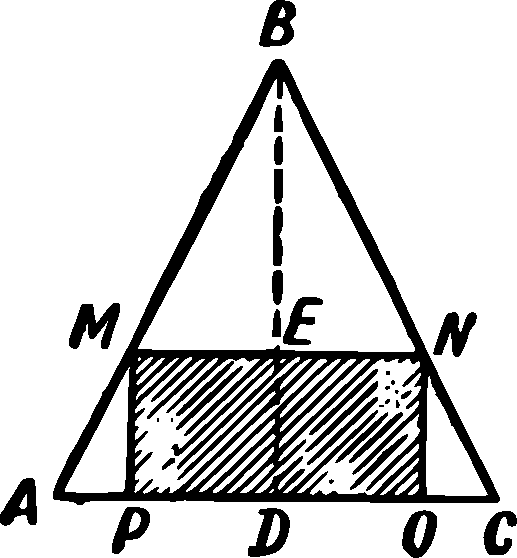
\includegraphics[width=\textwidth]{figures/ch-12/fig-182.pdf}
\sidecaption{To insert a rectangle of maximum area into a triangle.\label{fig-182}}
\end{marginfigure}


\ans Let $ABC$ be the given triangle (\figr{fig-182}), and $MNOP$ be the rectangle that should remain after cutting. From the similarity of triangles $ABC$ and $NBM$, we have:
\begin{equation*}%
\frac{BD}{BE} = \frac{AC}{NM},
\end{equation*}
hence
\begin{equation*}%
NM =  \frac{BE \cdot AC}{BD}.
\end{equation*}
Denoting one side $NM$ of the sought rectangle by $y$, its distance $BE$ from the vertex of the triangle by $x$, the base $AC$ of the given triangle by $a$, and its height $BD$ by $h$, we rewrite the previously obtained expression in the following form:
\begin{equation*}%
y = \frac{ax}{h}.
\end{equation*}
The area $S$ of the sought rectangle $MNOP$ is equal to:
\begin{align*}%
S &= MN \cdot NO = MN \cdot (BD - BE) \\
& = (h - x)y = (h - x)\frac{ax}{h},
\end{align*}
therefore,
\begin{equation*}%
\frac{Sh}{a} = (h - x)x.
\end{equation*}
The area $S$ will be maximum when the product $Sh / a $ is maximum, and consequently, when the product of the factors $(h - x)$ and $x$ reaches its maximum value. But the sum $h - x + x = h$ is a constant value. Hence, the product is maximum when
\begin{equation*}%
h - x = x,
\end{equation*}
hence
\begin{equation*}%
x = h/2.
\end{equation*}
We find that the side $MN$ of the sought rectangle passes through the midpoint of the triangle's height, and consequently, connects the midpoints of its sides. Therefore, this side of the rectangle is equal to $a/2$, and its other side is equal to $h/2$.


\section{The Tinsmith's Dilemma}
\label{sec-12.13}

\ques A tinsmith was asked to make a box without a lid from a square sheet of tin 60 cm wide, with the condition that the box should have the maximum possible capacity. The tinsmith pondered for a long time about the width to which the edges should be folded, but could not come to a definite solution (\figr{fig-183}). Perhaps the reader can help solve his dilemma?

\begin{figure}[h!]
\centering
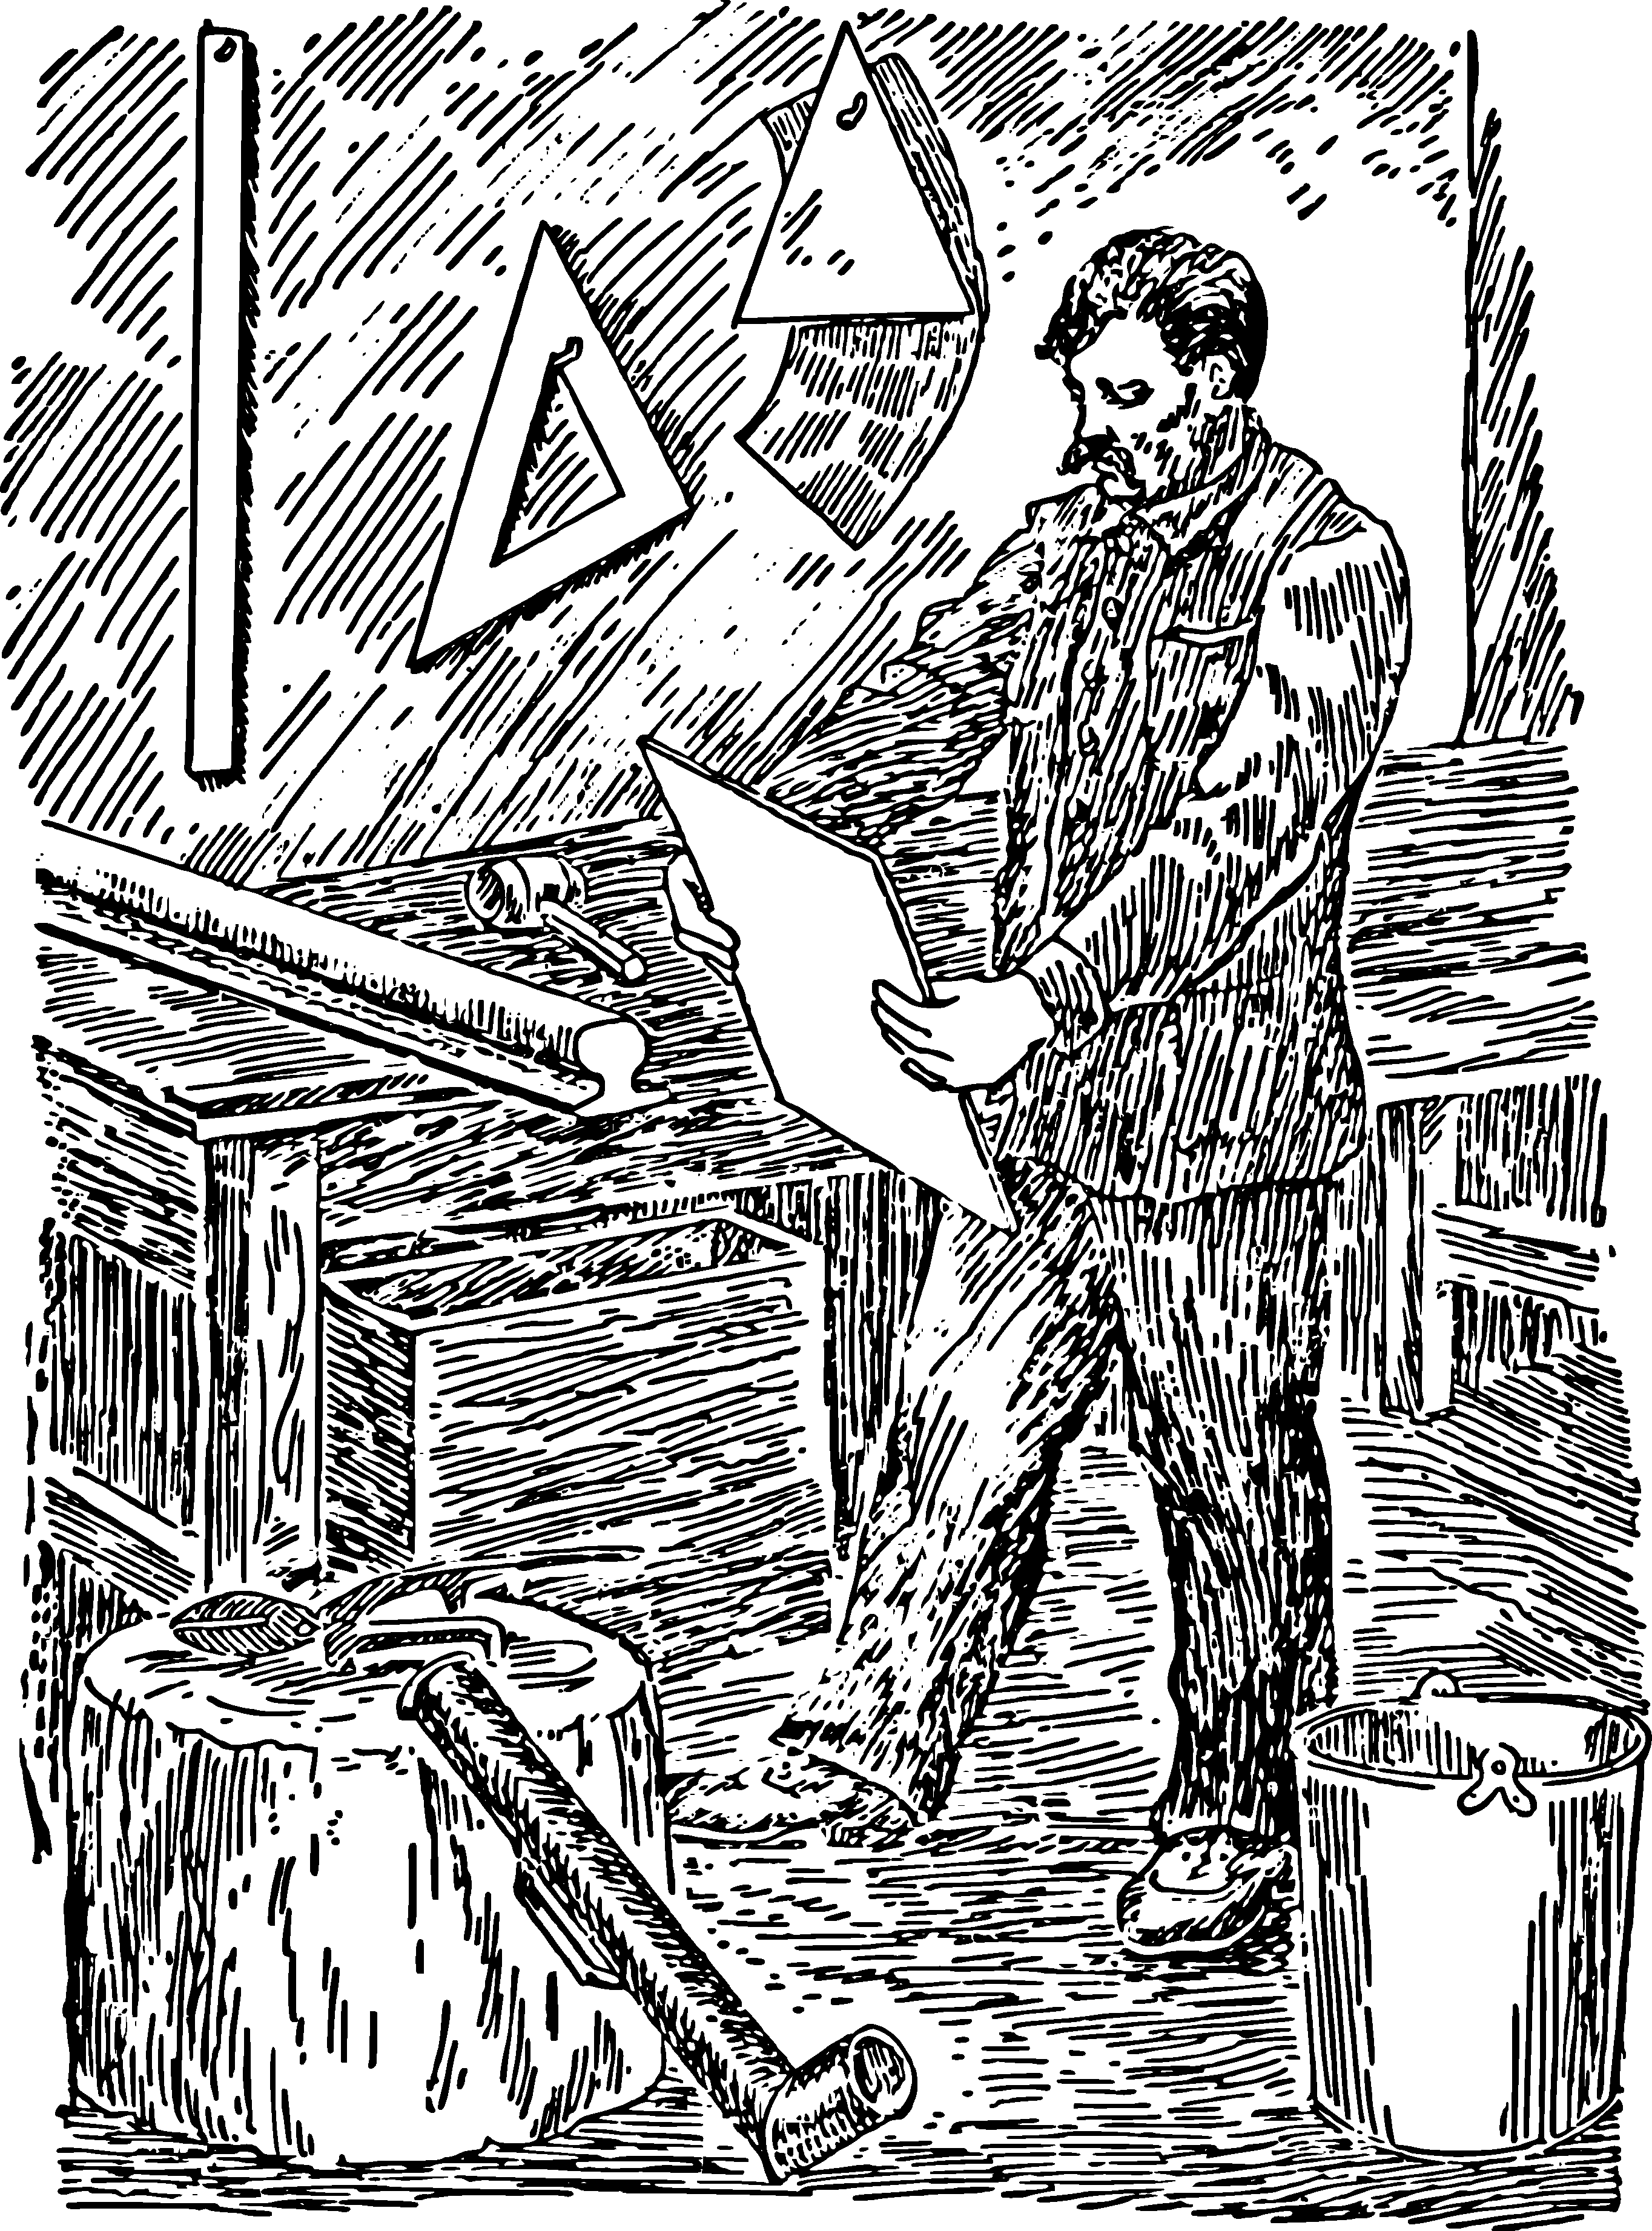
\includegraphics[width=0.8\textwidth]{figures/ch-12/fig-183.pdf}
\sidecaption{The tinsmith's dilemma.\label{fig-183}}
\end{figure}



\ans Let the width of the folded strips be $x$ (\figr{fig-184}). Then the width of the square base of the box will be $60 - 2x$, and the volume $V$ of the box can be expressed as:
\begin{equation*}%
v = (60 - 2x)(60 - 2x)\, x.
\end{equation*}
At what $x$ does this product have the greatest value? If the sum of the three factors were constant, the product would be greatest when they are equal. However, in this case, the sum of the factors
\begin{equation*}%
60 - 2x + 60 - 2x + x = 120 - 3x,
\end{equation*}
is not a constant value, as it changes with $x$. However, it is not difficult to make the sum of the three factors constant: it is enough to multiply both parts of the equation by 4. We get:
\begin{equation*}%
4v = (60 - 2x)(60 - 2x)4x.
\end{equation*}
The sum of these factors is
\begin{equation*}%
60 - 2x + 60 - 2x + 4x = 120
\end{equation*}
a constant value. Hence, the product of these factors reaches its maximum value when they are equal, i.e., when
\begin{equation*}%
60 - 2x = 4x,
\end{equation*}
from which 
\begin{equation*}%
x = 10.
\end{equation*}
Then \(4v \), and therefore \(v \), reach their maximum.
\begin{marginfigure}%[-3cm]%[h!]
\centering
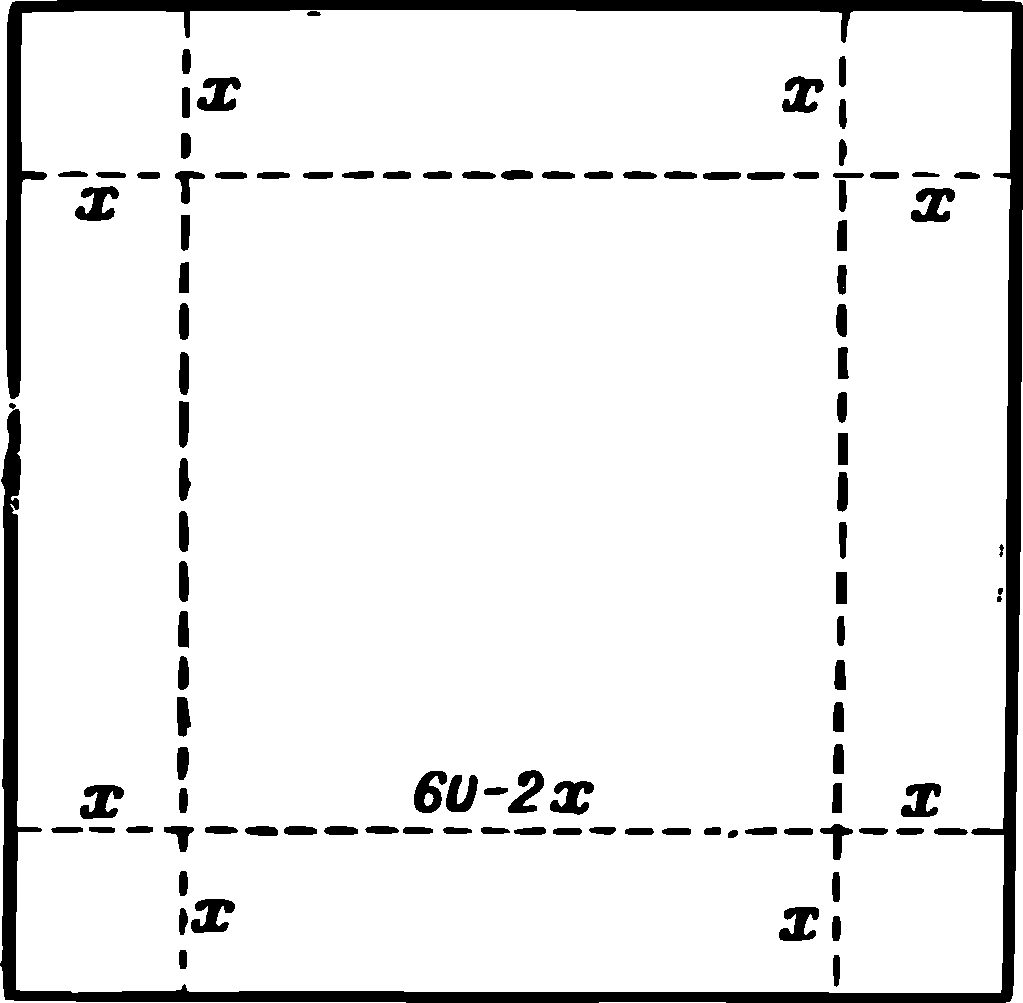
\includegraphics[width=\textwidth]{figures/ch-12/fig-184.pdf}
\sidecaption{Solution to the tinsmith's problem.\label{fig-184}}
\end{marginfigure}

Thus, the box will have the greatest volume if the edges of the tin sheet are folded to 10 cm. This maximum volume is equal to \(40 \times 40 \times 10 = \SI{16000}{\centi\meter\cubed}\). Folding 1 cm more or less will decrease the volume of the box in both cases. Indeed,
\begin{align*}%
9 \times 42 \times 42 & = \SI{15900}{\centi\meter\cubed}\\
11 \times 38 \times 38 & = \SI{15900}{\centi\meter\cubed}
\end{align*}
both of which are less than \SI{16000}{\centi\meter\cubed}.\sidenote[][2cm]{Solving the problem in general, we find that for a square sheet of width \(a\), to obtain a box with the maximum volume, the strips of width \(x = a/6 \) should be folded, because the product \((a - 2x)(a - 2x)x\), or \((a - 2x)(a - 2x)4x\), is greatest when \(a - 2x = 4x\).}


\section{The Turner's Dilemma}
\label{sec-12.14}



\ques A turner is given a cone and tasked with turning it into a cylinder so that as little material as possible is removed (\figr{fig-185}).


\begin{figure}[h!]
\centering
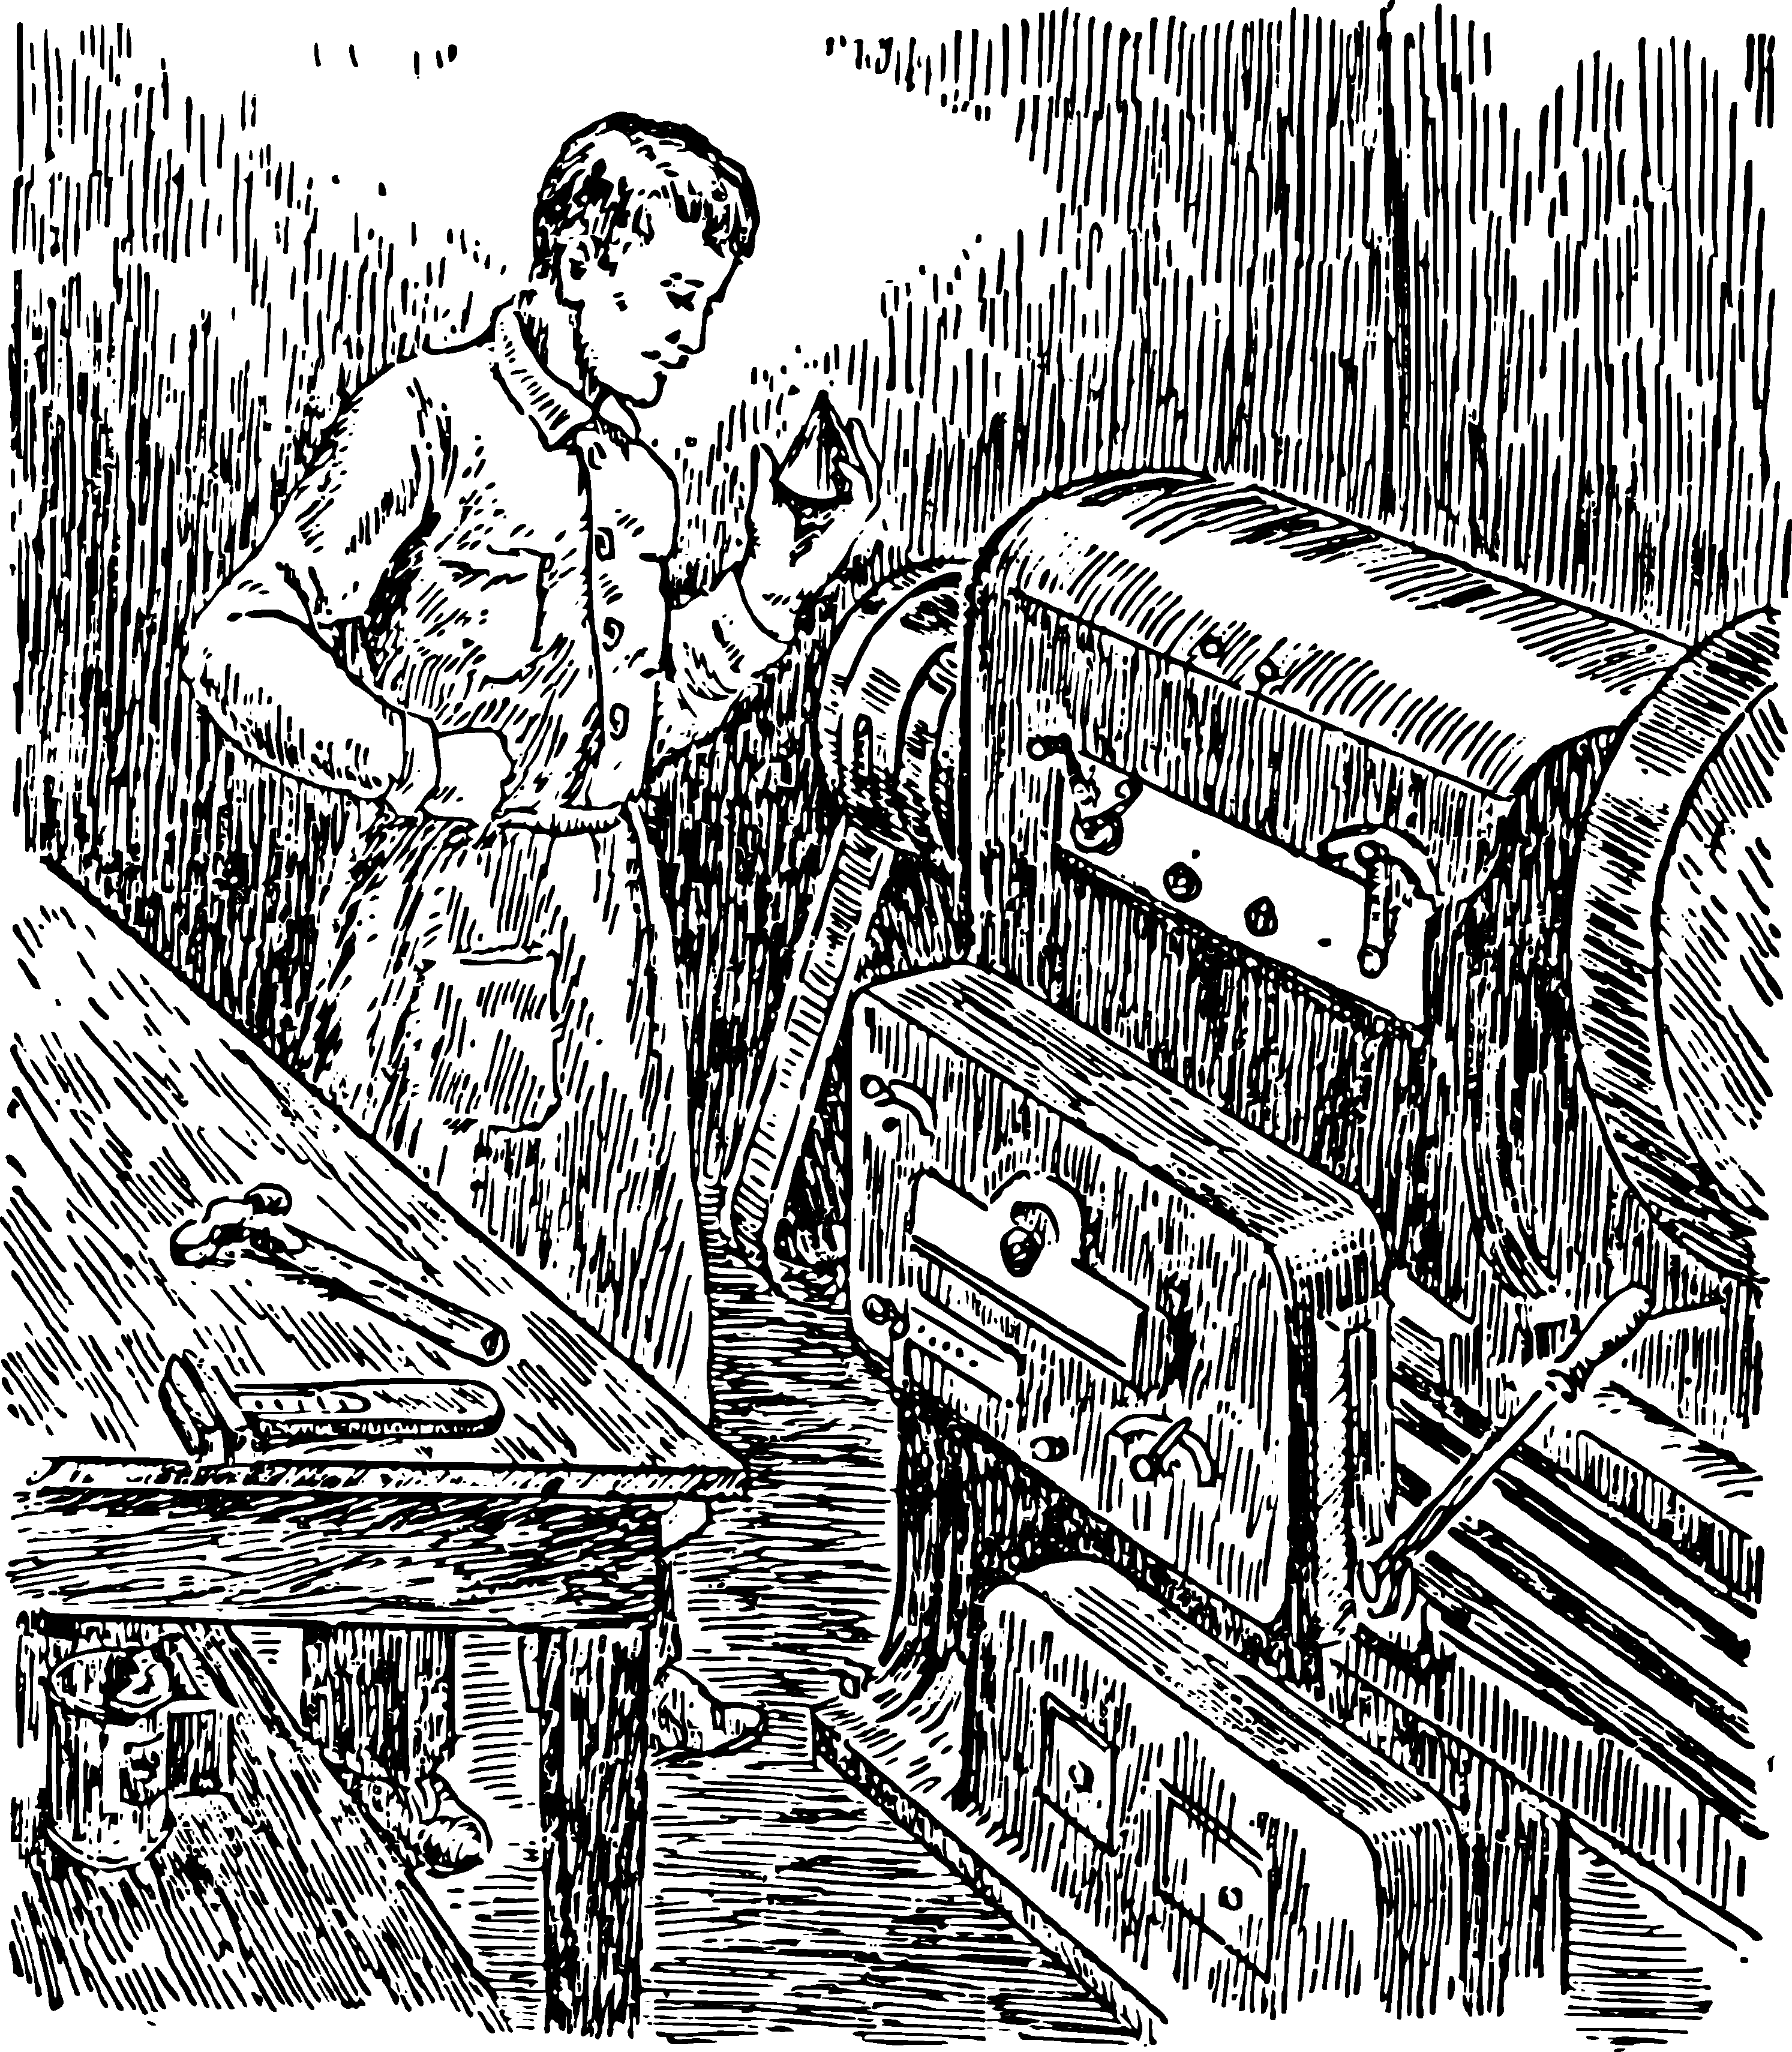
\includegraphics[width=0.8\textwidth]{figures/ch-12/fig-185.pdf}
\sidecaption[][-7cm]{The turner's dilemma.\label{fig-185}}
\end{figure}

The turner pondered the shape of the desired cylinder: should it be tall but narrow (\figr{fig-186}) or wide but short (\figr{fig-187}). He could not decide for a long time what shape would result in the cylinder with the largest volume, i.e., with the least amount of material removed. What should he do?





\ans The problem requires careful geometric consideration. Let $ABC$ (\figr{fig-188}) be the cross-section of the cone, $BD$ its height, denoted as $h$; the radius of the base $AD = DC$ denoted as $R$. The cylinder that can be turned from the cone has a cross-section $MNOP$. We need to find at what distance $BE = x$ from the vertex $B$ the top base of the cylinder should be located so that its volume is maximised.

\begin{marginfigure}[-7cm]%[h!]
\centering
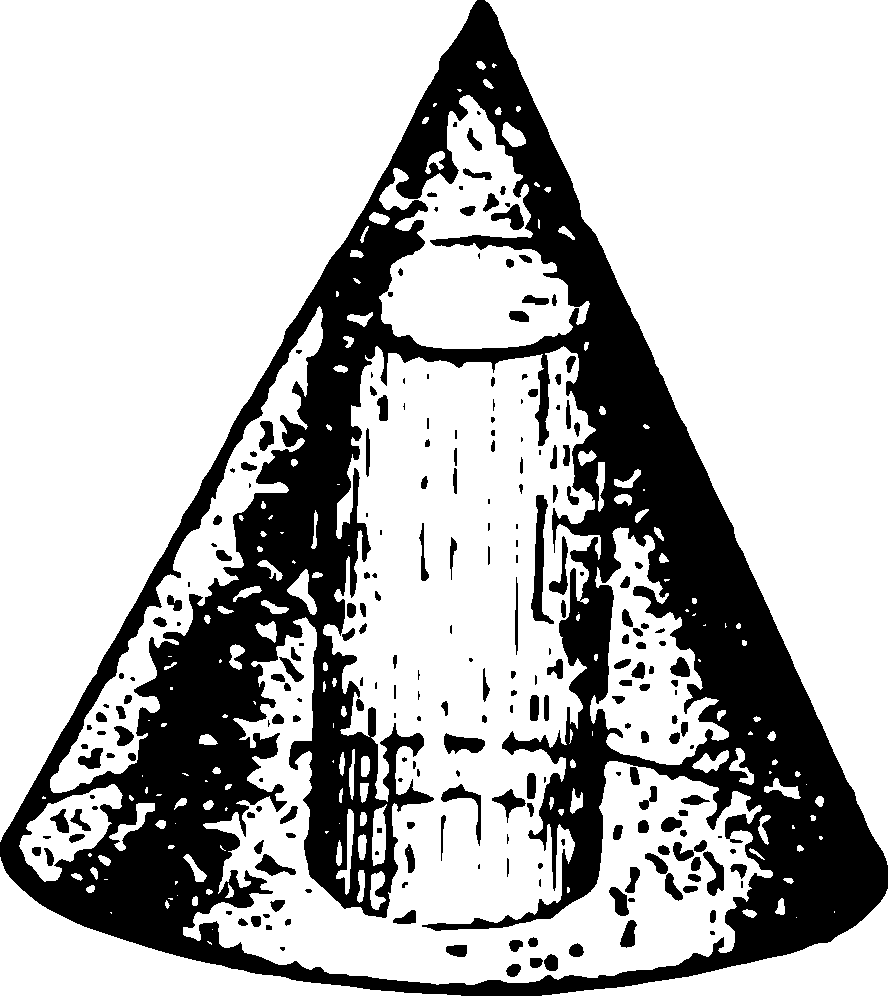
\includegraphics[width=0.8\textwidth]{figures/ch-12/fig-186.pdf}
\sidecaption{A cylinder can be turned from the cone to be tall but narrow or wide but short. In which case will less material be removed?\label{fig-186}}
\end{marginfigure}
The radius \( r \) of the base of the cylinder ($PD$ or $ME$) is easily found from the proportion:
\begin{align*}% 
\frac{ME}{AD} & = \frac{BE}{BD} \,\, \text{i.e.,}\\
\frac{r}{R} & = \frac{x}{h} \,\, \text{from which,}\\
 r & = \frac{Rx}{h}.
\end{align*}
\begin{marginfigure}[-4cm]%[h!]
\centering
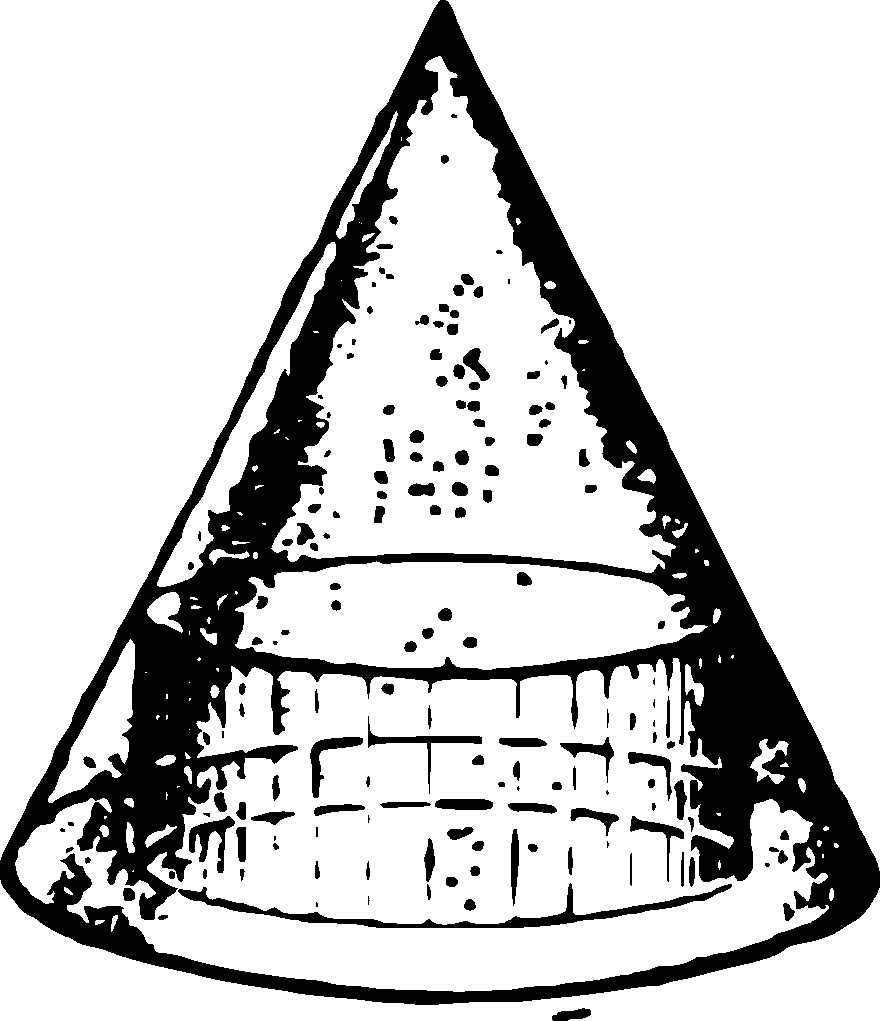
\includegraphics[width=0.8\textwidth]{figures/ch-12/fig-187.pdf}
\sidecaption{A cylinder can be turned from the cone to be tall but narrow or wide but short. In which case will less material be removed?\label{fig-187}}
\end{marginfigure}
The height $ED$ of the cylinder is equal to \( h - x \). Consequently, its volume is
\begin{equation*}%
 v = \pi \left(\frac{Rx}{h}\right)^{2} (h - x) = \pi \frac{R^{2} x^{2}}{h^{2}} (h - x). 
\end{equation*}
from which
\begin{equation*}%
v \frac{h^{2}}{\pi R^{2}} = x^{2} (h - x).
\end{equation*}
\begin{marginfigure}[-2cm]%[h!]
\centering
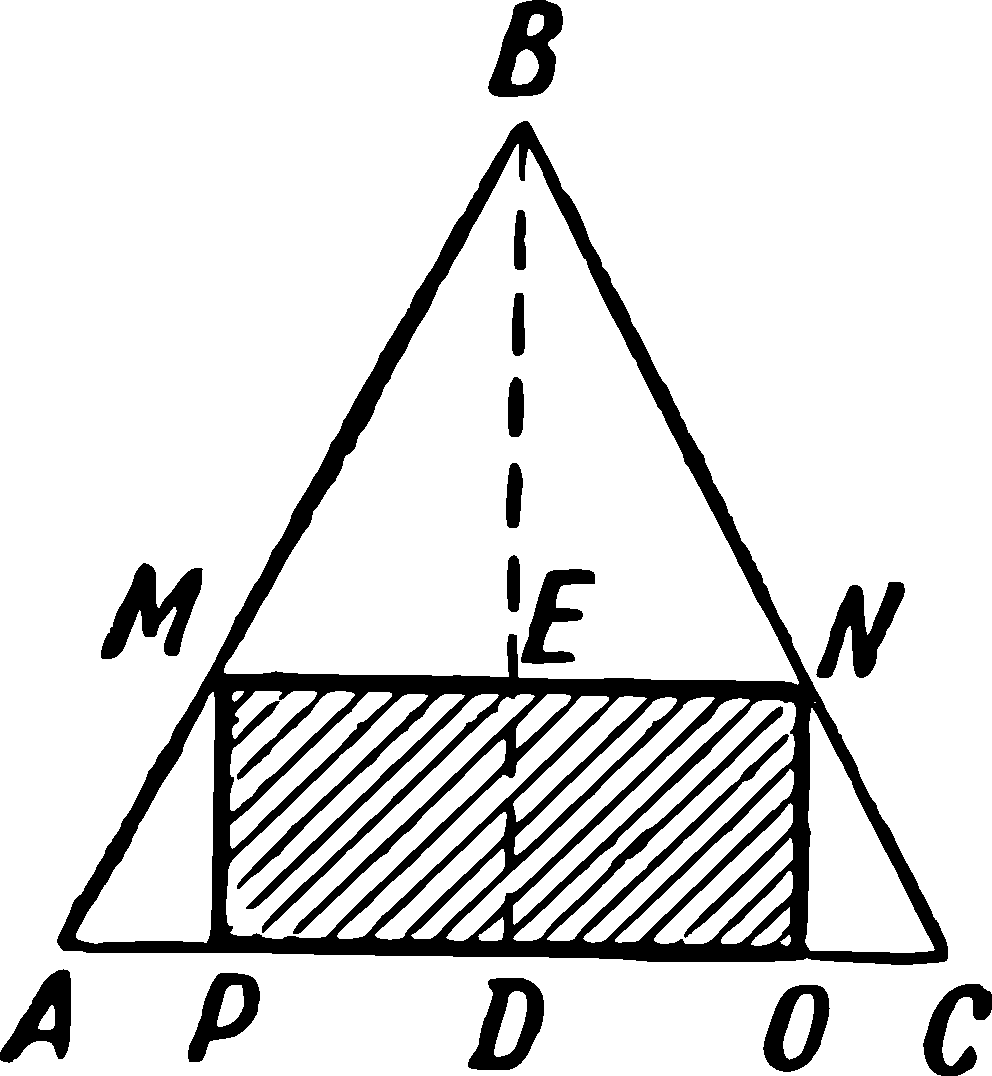
\includegraphics[width=0.8\textwidth]{figures/ch-12/fig-188.pdf}
\sidecaption{Axial section of the cone and the cylinder.\label{fig-188}}
\end{marginfigure}
In the expression \( vh^{2}/\pi R^{2}\), the values \(h\), \( \pi \), and \(R \) are constants, and only \(v \) is a variable. We want to find such an \(x \) for which \(v \) becomes the greatest. But obviously, \(v \) will be the greatest at the same time as \(vh^{2}/\pi R^{2}\), that is, \(x^{2} \, (h - x)\). When does this latter expression become the greatest? Here, we have three variable factors: \(x\), \(x\), and \((h - x)\). If their sum were constant, the product would be greatest when the factors were equal. This constancy of the sum is easy to achieve if both parts of the last equation are multiplied by 2. Then we get:
\begin{equation*}%
2 \frac{vh^{2}}{\pi R^{2}} = x^{2} \,(2h - 2x).
\end{equation*}
Now the three factors on the right side have a constant sum:
\begin{equation*}%
x + x + 2h - 2x = 2h.
\end{equation*}
Therefore, their product will be the greatest when all the factors are equal, that is,
\begin{equation*}%
x = 2h - 2x, \qand x = \frac{2h}{3}.
\end{equation*}
Then the expression \(2vh^2/\pi R^{2}\) will also be maximised, and with it the volume of the cylinder.

Now we know how the desired cylinder should be turned: its upper base should be located at 2/3 of the cone's height from the vertex.


\section{How to Lengthen a Board?}
\label{sec-12.15}

When making something in a workshop or at home, it sometimes happens that the material at hand does not have the required dimensions.

In such cases, it is worth attempting to modify the material's dimensions through appropriate processing, and much can be achieved with some geometric and construction ingenuity and calculation.


\begin{figure}[h!]
\centering
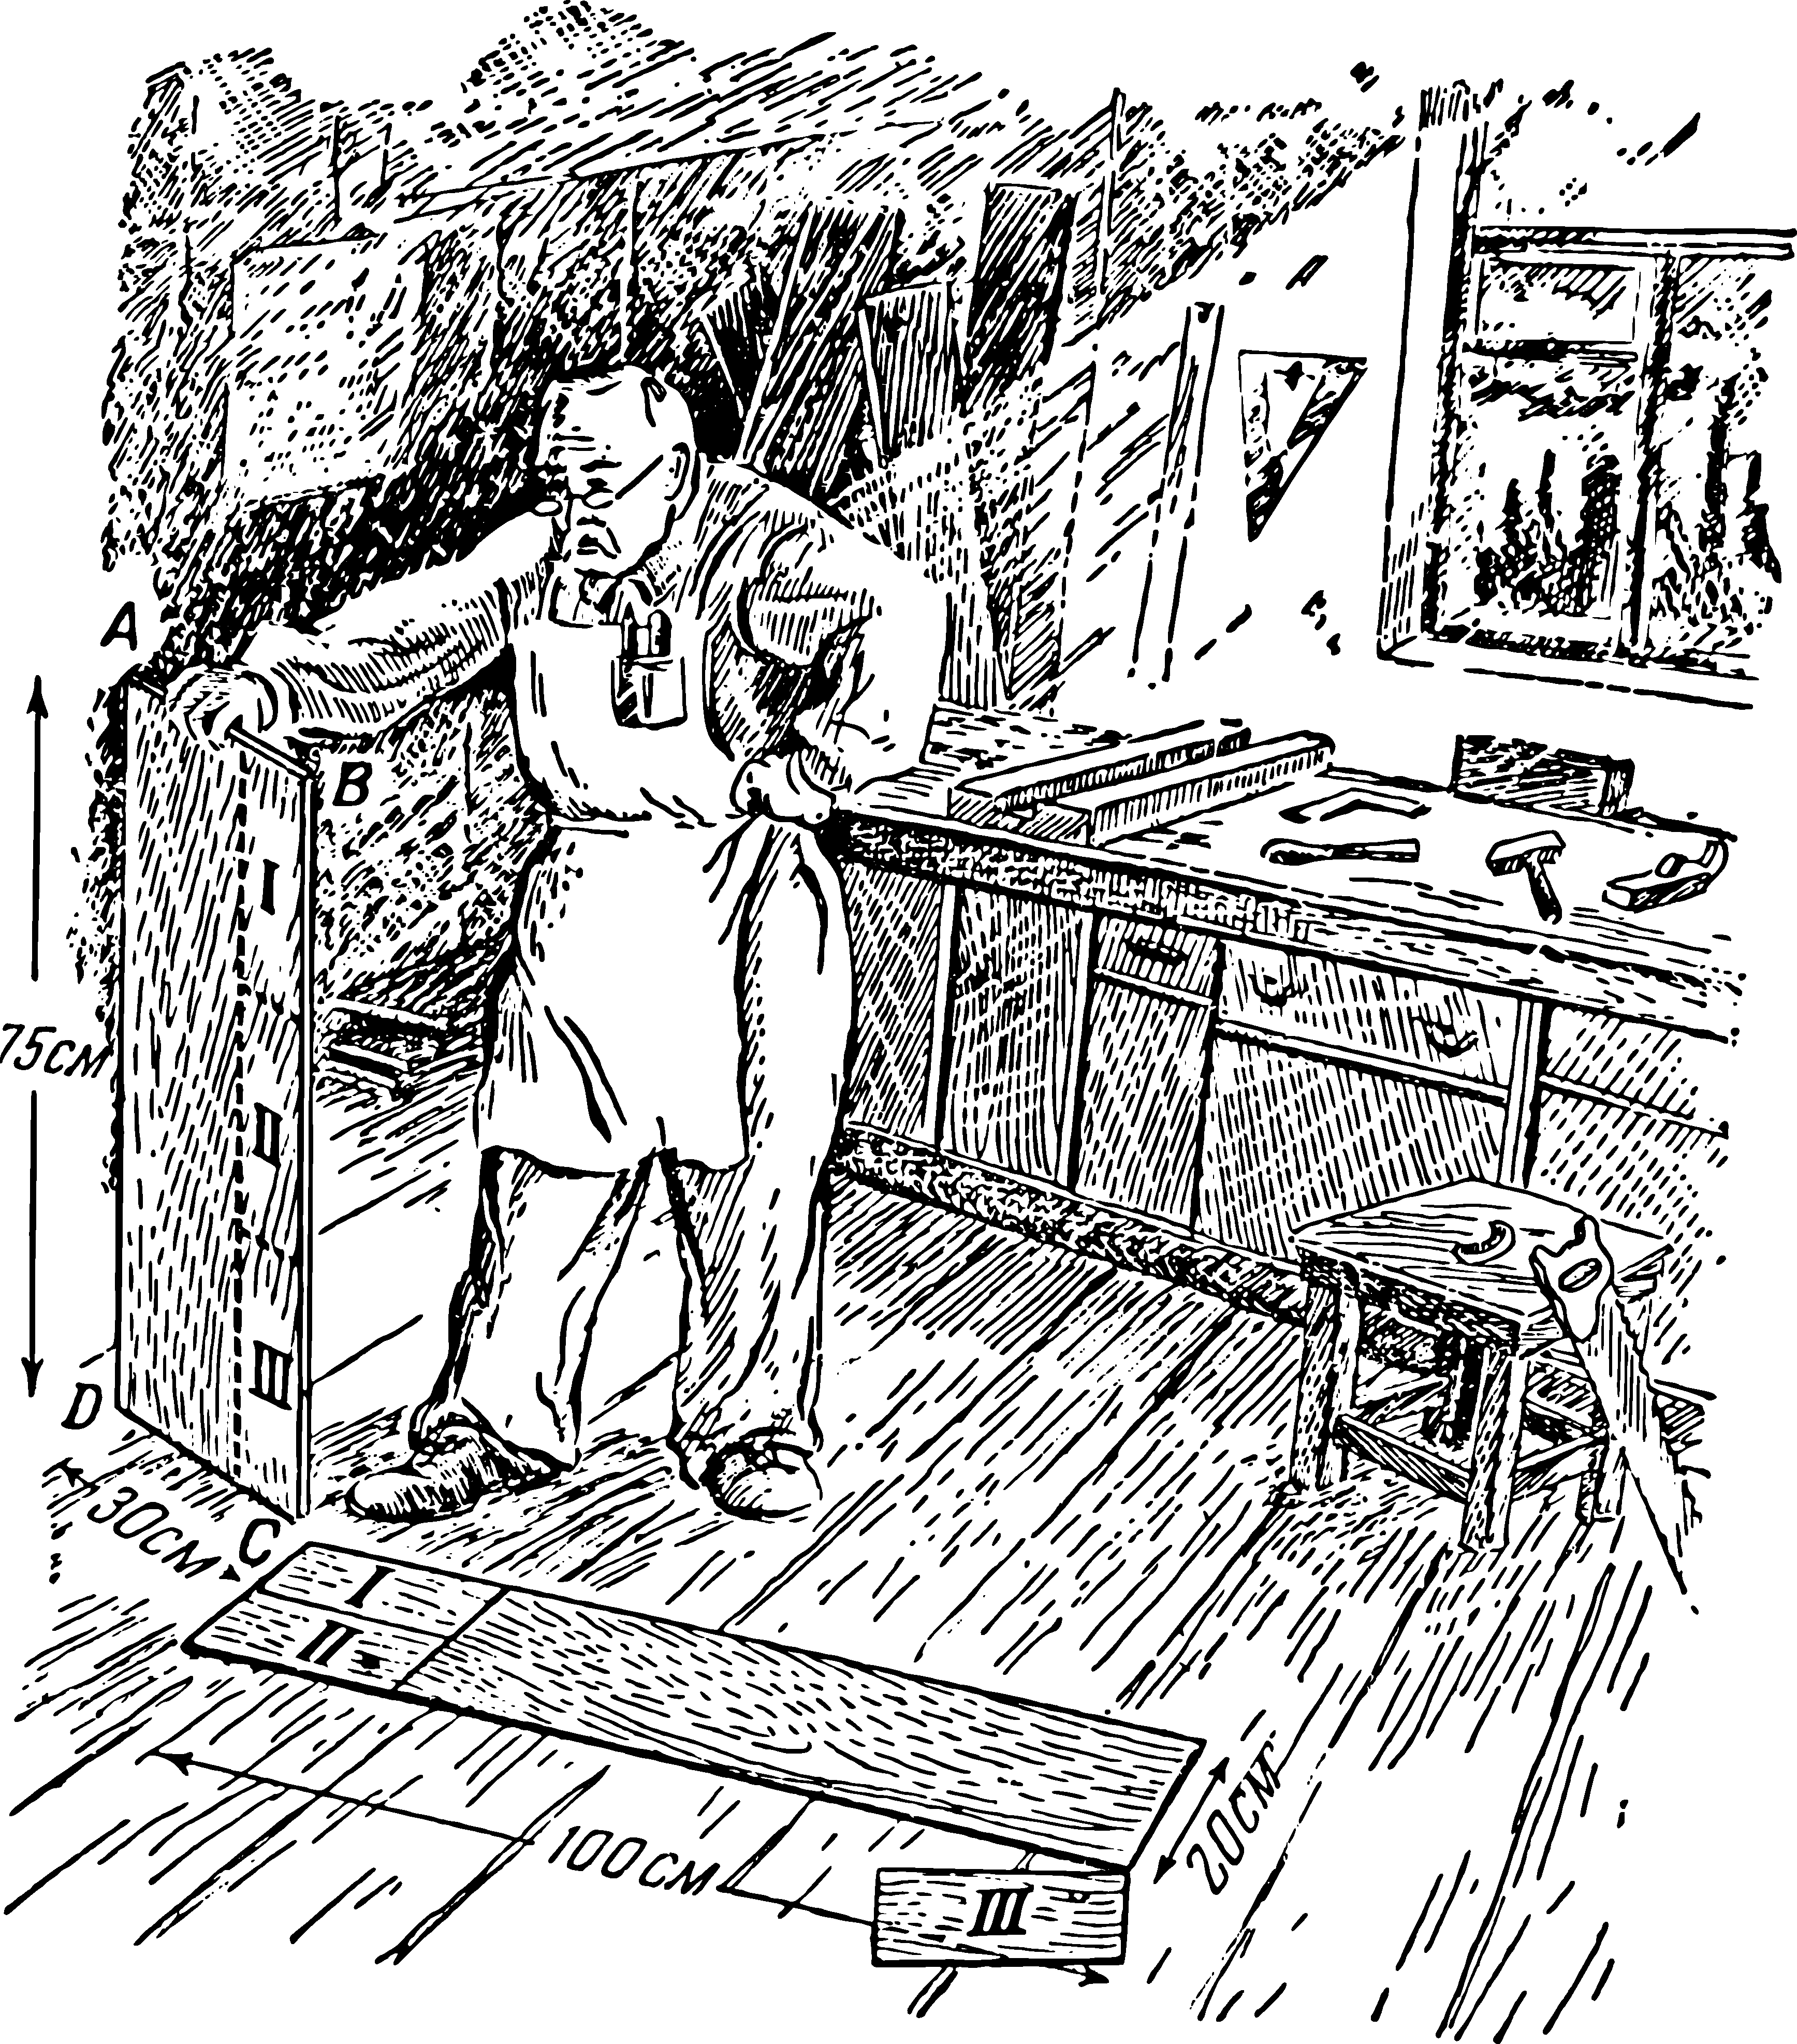
\includegraphics[width=0.8\textwidth]{figures/ch-12/fig-189.pdf}
\sidecaption{How to lengthen the board by means of three sawing and one gluing?\label{fig-189}}
\end{figure}
 

Imagine this situation: you need a board of precise dimensions for making a bookshelf, specifically, 1 meter in length and 20 centimetres in width, but you have a shorter yet wider board, for example, 75 centimetres in length and 30 centimetres in width (see \figr{fig-189} on the left).

What should you do?
\begin{marginfigure}%[-2cm]%[h!]
\centering
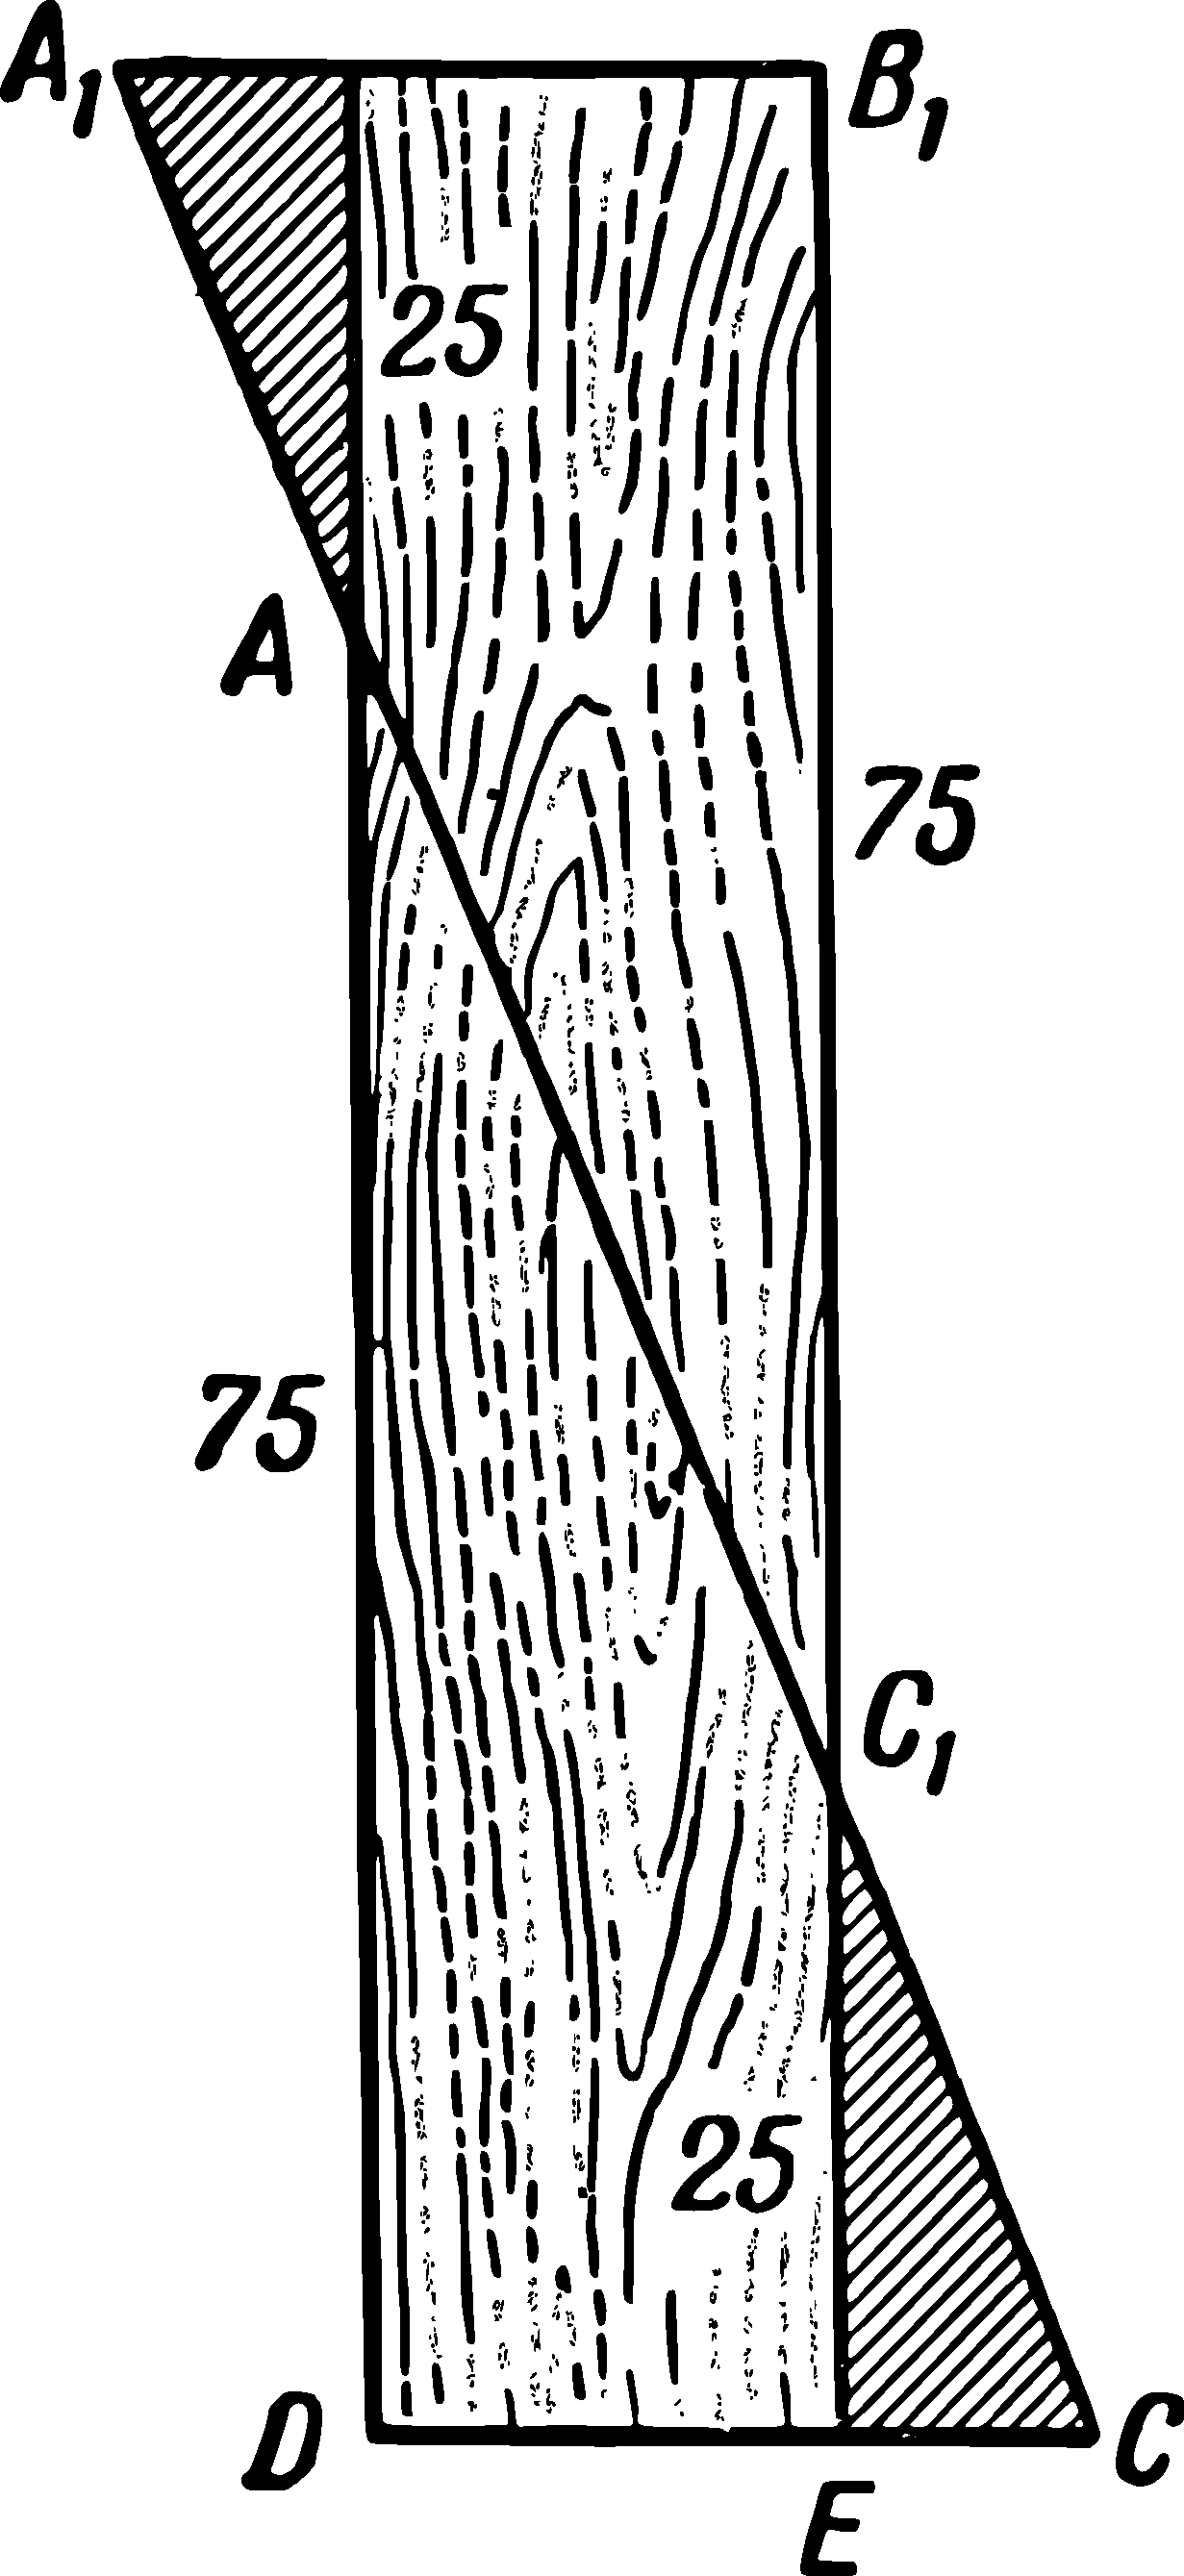
\includegraphics[width=0.7\textwidth]{figures/ch-12/fig-190.pdf}
\sidecaption{Solving the problem of lengthening the board.\label{fig-190}}
\end{marginfigure}

Of course, you could saw off a strip 10 centimetres wide along the length of the board (dashed line), cut it into three equal pieces each 25 centimetres long, and use two of them to extend the board (see \figr{fig-189} at the bottom).

This solution would be inefficient in terms of the number of operations (three cuts and three gluing points) and would not satisfy the strength requirements (strength would be reduced at the points where the strips are glued to the board).


You need to (see \figr{fig-190}) cut the board $ABCD$ along the diagonal $AC$ and shift one half (for example, $ABC$) along the diagonal, parallel to itself, by the distance $C_{1}E$, which equals the missing length, i.e., 25 cm. The total length of the two halves will then be 1 meter. Now these halves need to be glued along the line $AC_{1}$, and the excess (shaded triangles) should be cut off. This will result in a board of the required dimensions.

Indeed, from the similarity of triangles $ADC$ and $C_{1}EC$, we have:
\begin{align*}%
\frac{AD}{DC} & = \frac{C_{1}E}{EC},\, \, \text{from which}\\
EC & = \frac{DC}{AD} \times C_{1}E, \qor \\
EC & = \frac{30}{75} \times 25 = \SI{10}{\centi\meter};\\
DE & = DC - EC =  \SI{30}{\centi\meter} -  \SI{10}{\centi\meter} =  \SI{20}{\centi\meter}.
\end{align*}



\section{The Shortest Path}
\label{sec-12.15}

In conclusion, let’s consider a problem of ``maxima and minima'', which can be solved with a very simple geometric construction.


\ques Along the bank of a river, a water tower needs to be built to supply water via pipes to villages $A$ and $B$ (see \figr{fig-191}).


\begin{figure}[h!]
\centering
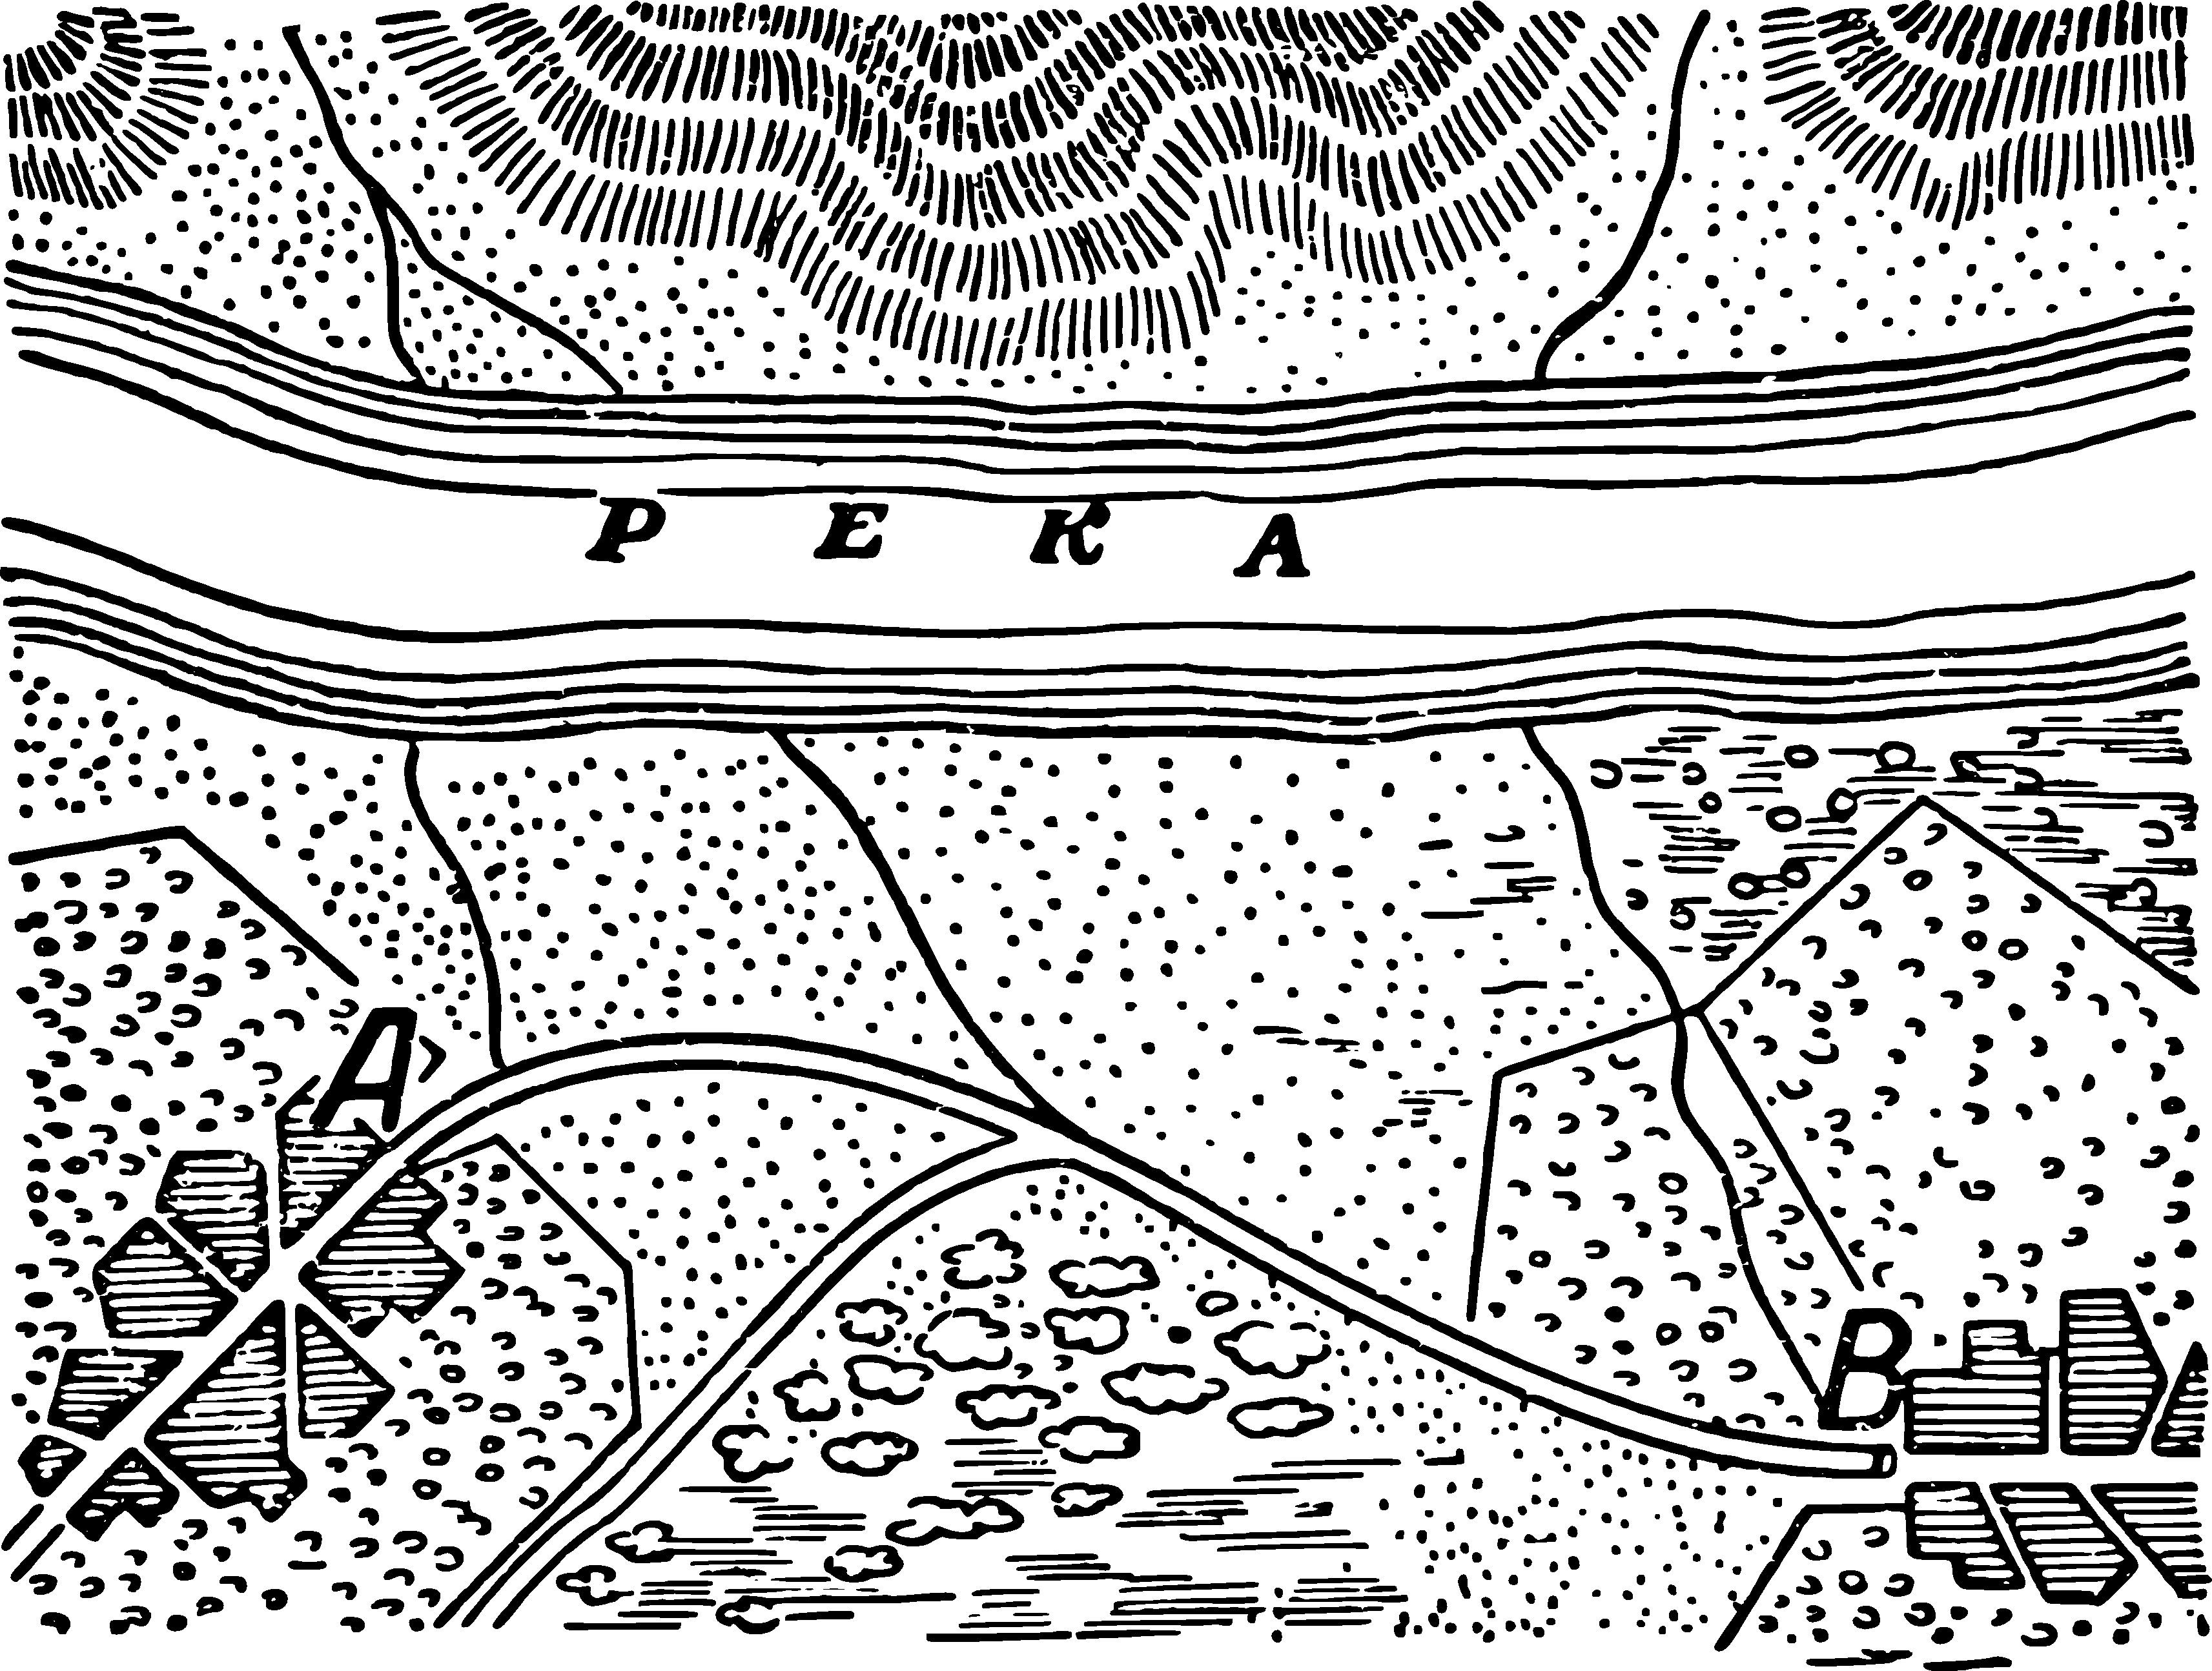
\includegraphics[width=0.9\textwidth]{figures/ch-12/fig-191.pdf}
\sidecaption{The problem of the water tower.\label{fig-191}}
\end{figure}


Where should it be built so that the total length of the pipes from the tower to both villages is the shortest?

\ans The problem reduces to finding the shortest path from $A$ to the bank and then to $B$.

Suppose the shortest path is $ACB$ (see \figr{fig-191}). Fold the diagram along line $CN$. We get point $B'$. If $ACB$ is the shortest path, then, since $CB' = CB$, the path $ACB'$ must be shorter than any other (e.g., $ADB'$). Thus, to find the shortest path, we only need to locate the point $C$ where the straight line $AB'$ intersects the riverbank. Then, connecting $C$ and $B$, we find both parts of the shortest path from $A$ to $B$.

\begin{figure}%[-2cm]%[h!]
\centering
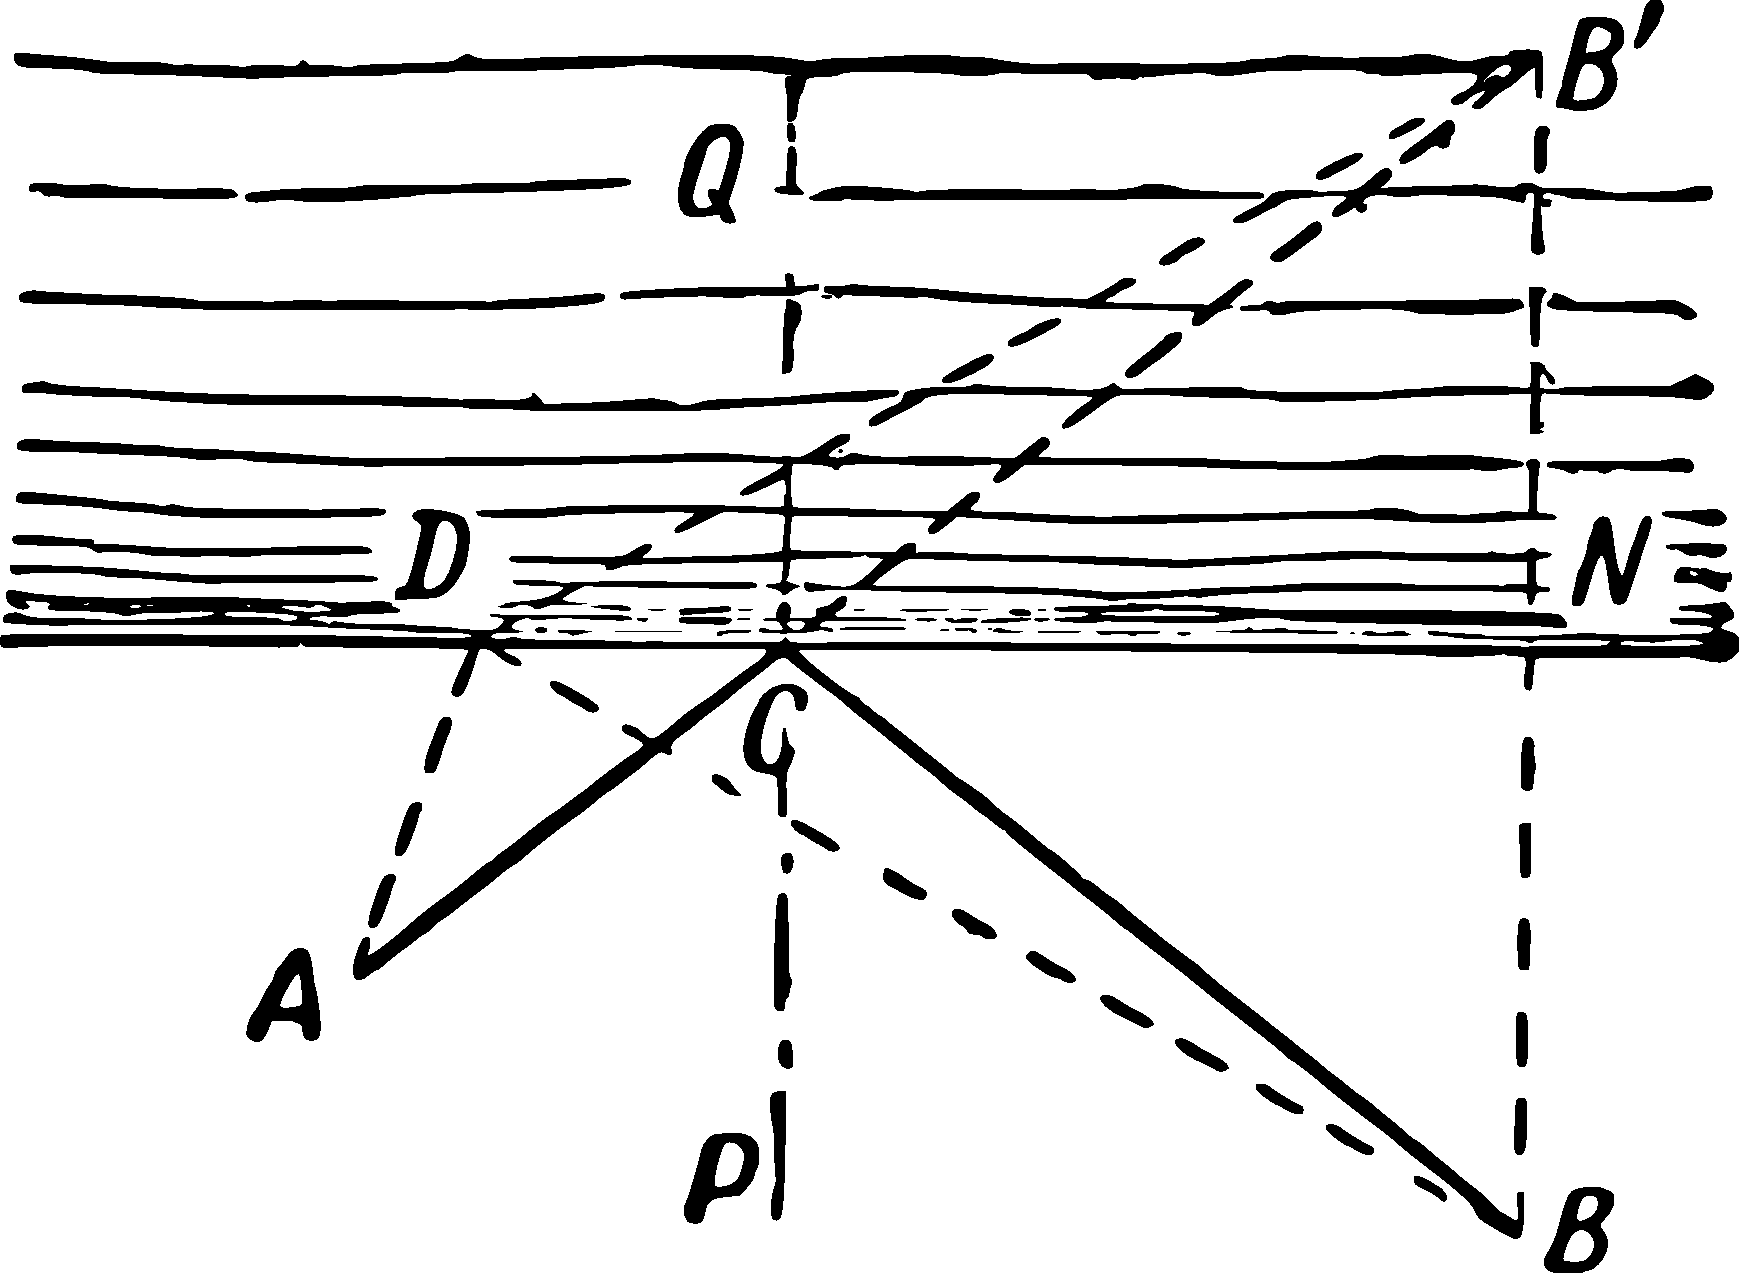
\includegraphics[width=0.7\textwidth]{figures/ch-12/fig-192.pdf}
\sidecaption{Geometric solution to the problem of finding the shortest path.\label{fig-192}}
\end{figure}


By drawing a perpendicular at point $C$ to $CN$, it's easy to see that the angles $ACP$ and $BCP$, formed by both parts of the shortest path with this perpendicular, are equal $(\angle ACP = \angle B'CQ = \angle  BCP)$.

This is known as the law of reflection of a light ray off a mirror: the angle of incidence equals the angle of reflection. Hence, a light ray chooses the shortest path when it reflects, a conclusion known to the ancient physicist and geometer Heron of Alexandria two thousand years ago.




\begin{center}
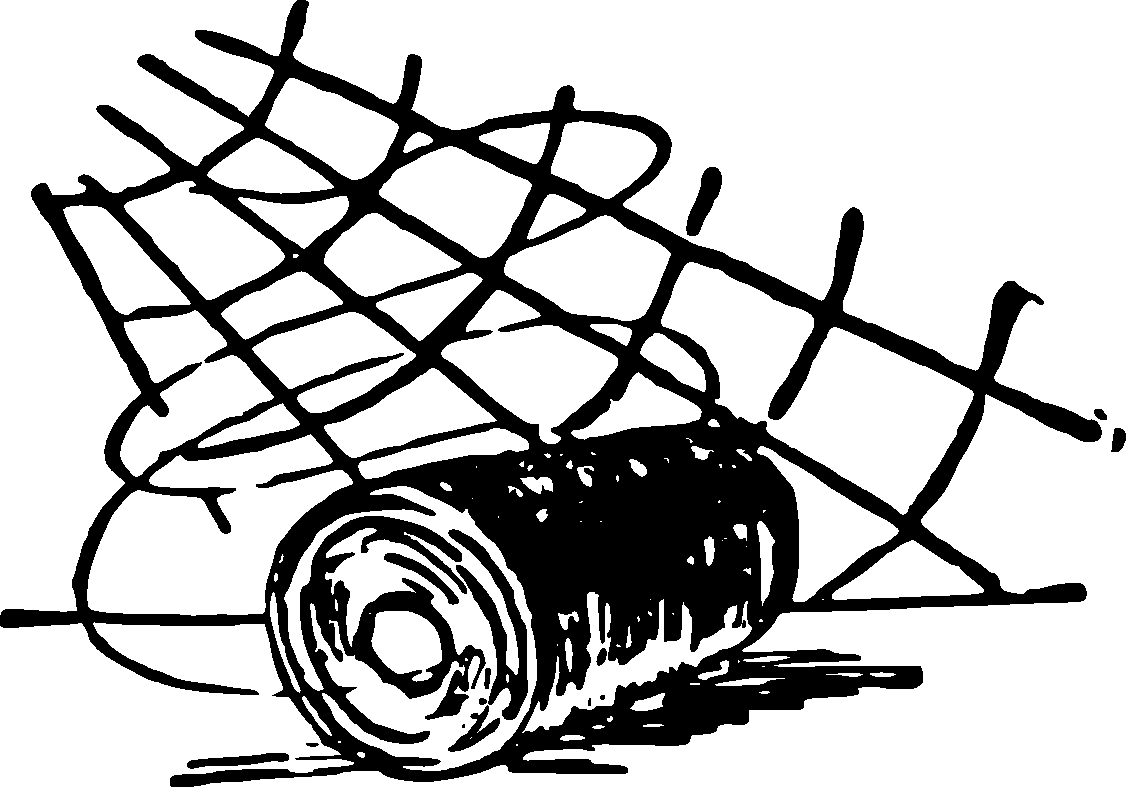
\includegraphics[width=0.3\textwidth]{figures/ch-11/fig-ch-11-tail.pdf}
\end{center}


















